\documentclass[10pt, conference]{IEEEtran}
\usepackage{graphicx}
\usepackage{amsmath}
\usepackage{amssymb}
\usepackage{booktabs}
\usepackage{tabularx}
\usepackage{caption}
\usepackage{subcaption}
\usepackage{cite}
\usepackage{xcolor}
\usepackage{array}
\usepackage{multirow}
\usepackage{enumitem}
\usepackage{balance}
\usepackage{placeins}
\usepackage{dblfloatfix}
\usepackage{float}
\usepackage[hidelinks]{hyperref}

\setlength{\textfloatsep}{10pt plus 3pt minus 2pt}
\setlength{\floatsep}{10pt plus 3pt minus 2pt}
\setlength{\intextsep}{10pt plus 3pt minus 2pt}
\setlength{\dbltextfloatsep}{10pt plus 3pt minus 2pt}
\setcounter{topnumber}{10}
\setcounter{bottomnumber}{10}
\setcounter{totalnumber}{20}
\setcounter{dbltopnumber}{10}
\renewcommand{\topfraction}{0.95}
\renewcommand{\bottomfraction}{0.95}
\renewcommand{\textfraction}{0.05}
\renewcommand{\floatpagefraction}{0.90}
\renewcommand{\dbltopfraction}{0.95}
\renewcommand{\dblfloatpagefraction}{0.90}

\renewcommand{\thesection}{\Roman{section}}
\renewcommand{\thesubsection}{\thesection-\Alph{subsection}}

\title{Automatic Vehicle Gate Access System Using Weather-Aware Preprocessing, YOLOv8n License Plate Recognition, and EfficientNet-B4 Make--Model Verification}

\author{\IEEEauthorblockN{Abdul Hadi, Ali Raza Chaudhry, and Abdullah Yaseen}
\IEEEauthorblockA{Department of Computer Engineering\\
COMSATS University Islamabad, Lahore Campus\\
Lahore, Pakistan\\
Supervisor: Dr.\ Taimoor Naeem\\
B.S.\ Computer Engineering}}

\begin{document}
\emergencystretch=2em
\graphicspath{{figures/}{figures/lpd/}{figures/pre/}{figures/lpr_char/}{figures/vmmr/}{figures/hw/}{figures/dashboard/}}
\maketitle

\begin{abstract}
Manual gate checks and plate-only automatic number plate recognition (ANPR) are slow, error-prone, and vulnerable to plate swapping. This paper presents the implemented Automatic Vehicle Gate Access System developed as an undergraduate final-year project: a weather-aware classical preprocessing front end, a two-stage YOLOv8n license plate recognition (LPR) pipeline, and an EfficientNet-B4 vehicle make and model recognizer (VMMR) over 245 classes, fused by a dual-modality authorization policy and monitored through a cloud web dashboard. Fog and haze are mitigated with a dark-channel prior and guided filtering; rain streaks are suppressed with multi-scale vertical median filtering and Telea inpainting under an edge-protection mask; night frames are enhanced with LAB-space CLAHE. On the reported project benchmarks, YOLOv8n plate detection reaches mAP@0.5 of 98.07\% (precision 98.50\%, recall 95.53\%) after 50 epochs; the 38-class character detector reports mAP@0.5 of 97.7\% after 100 epochs under mirrored training validation (explicitly flagged); and EfficientNet-B4 achieves 96.24\% Top-1 accuracy on 17{,}254 held-out test images. All three models run locally on an Orange Pi~5 Pro (16\,GB) from a USB 1080p camera, with measured end-to-end latency of about 700--1000\,ms per frame, and events sync to a React dashboard hosted on Vercel. All project figures from the \texttt{figures/} folder are included at full page width for readability.
\end{abstract}

\begin{IEEEkeywords}
Automatic number plate recognition, vehicle make and model recognition, YOLOv8, EfficientNet, dark channel prior, rain removal, CLAHE, edge AI, access control.
\end{IEEEkeywords}

\section{Introduction}
\label{sec:intro}
Vehicle access control at campuses, gated communities, and parking facilities still often depends on manual inspection or physical credentials such as RFID tags and barcodes. These methods do not scale well under peak traffic, are easy to misuse when credentials are shared or lost, and provide limited auditability. Camera-based ANPR offers contactless identification, but outdoor gates introduce fog, rain, glare, and low light that degrade localization and reading. Plate-only decisions also fail when a cloned plate is mounted on an unauthorized vehicle.

This work implements a complete software--hardware gate prototype. The system combines weather-conditioned classical restoration, YOLOv8n plate localization and 38-class character detection with deterministic Pakistani plate formatting, EfficientNet-B4 fine-grained make--model classification over 245 classes, and dual-check authorization against a registered-vehicle store, with edge inference on an Orange Pi~5 Pro and cloud monitoring on Vercel. The contribution is engineering integration and experimental documentation of an end-to-end student deployment, not a new detector backbone.

\subsection{Problem Statement}
Given an RGB frame $I$ from a gate-lane camera, the system must recover a plate string $s$, predict a make--model class $y\in\{1,\ldots,245\}$, and return an access decision $a\in\{\textsc{allow},\textsc{deny},\textsc{temporary}\}$ by comparing $(s,y)$ with a registry $\mathcal{W}$. The same stack must remain usable when $I$ is degraded by fog, rain, or night illumination, which is addressed by restoring $\hat{I}$ before inference.

\subsection{Objectives}
\begin{itemize}[leftmargin=*,itemsep=1pt]
\item train a YOLOv8n license plate detector for gate-distance localization;
\item train a YOLOv8n character/digit detector (38 classes) with post-processing for regional plate tokens;
\item fine-tune EfficientNet-B4 for 245-way vehicle make and model classification;
\item apply fog, rain, and night preprocessing before recognition;
\item authorize access by cross-checking plate text and predicted vehicle identity;
\item meet a total response budget below 2\,s from capture to decision, with on-device CPU inference in the 700--1000\,ms range.
\end{itemize}

\subsection{Scope and Contribution}
Software scope covers the three AI modules, weather preprocessing, JSON-backed authorization, and a React/Node.js dashboard. Hardware scope covers Orange Pi~5 Pro (16\,GB), a USB 1080p camera, Wi-Fi upload, and optional GPIO/LED indication. Full industrial barrier-motor integration, snow removal, and automatic weather sensing are out of scope for this FYP cycle. Algorithmic novelty is not claimed beyond application-specific integration of established methods~\cite{he2009dcp,tan2019efficientnet,ultralytics2023yolov8}.

\section{Related Work}
\label{sec:related}
Classical ANPR pipelines used edge detection, morphology, and OCR engines. Modern systems replace hand-crafted stages with CNN detectors; YOLO-family models are widely used for plate localization~\cite{redmon2018yolov3,bochkovskiy2020yolov4,ultralytics2023yolov8}. Character reading may use OCR after cropping or a second detector that treats glyphs as objects~\cite{thapliyal2023alpr}. Fine-grained VMMR uses transfer learning from ImageNet; EfficientNet is a practical capacity/memory compromise~\cite{tan2019efficientnet}. Outdoor reliability depends on restoration such as the dark channel prior with guided filtering~\cite{he2009dcp,he2010guided,he2011dcp}, directional rain filtering with inpainting~\cite{telea2004}, and CLAHE on luminance~\cite{zuiderveld1994clahe}. This project documents one integrated campus-style pipeline rather than a new network family.

\section{System Architecture}
\label{sec:system}
Figures~\ref{fig:sys_overview}--\ref{fig:dash_arch} summarize the software architecture, updated block diagram, recognition stacks, edge hardware, and dashboard design. Figures~\ref{fig:admin_feed}--\ref{fig:edge_gui} document the role-based UI and Orange Pi deployment evidence used in the FYP demos.

\section{Proposed Methodology}
\label{sec:method}
\subsection{Weather-Aware Preprocessing}
Three classical branches restore frames before AI inference (Figs.~\ref{fig:pre_fog_in}--\ref{fig:pre_night_out}). Branch selection is software-flagged or manual; physical weather sensors are not yet attached.

\textbf{Fog/haze.} Dark-channel estimation uses a $13\times13$ morphological kernel. Atmospheric light is taken from the darkest 0.1\% of pixels. Transmission is refined with a guided filter (radius 50). Scene radiance recovery is followed by residual-haze cleanup, gray-world white balance, adaptive gamma $\gamma\in[0.6,1.8]$, CLAHE on luminance (clip 2.5, $8\times8$ tiles), HSV saturation gain $\times1.2$, bilateral denoising, and unsharp masking~\cite{he2009dcp,he2010guided}.

\textbf{Rain.} An edge-protection mask is built with bilateral smoothing and Canny edges. Multi-scale vertical median filters (kernels 15, 11, 7) suppress streaks with brightness-rejection blending. Remaining bright rain spots outside protected regions are filled with Telea inpainting (radius 3)~\cite{telea2004}.

\textbf{Night/low light.} Adaptive black-level lift is applied in LAB $L^\ast$, followed by CLAHE (clip 4.5--8.5, $6\times6$ tiles), adaptive gamma $\gamma\in[0.28,0.62]$, global gain when mean intensity is below 100, HSV saturation $\times1.55$, and unsharp masking~\cite{zuiderveld1994clahe}.

\subsection{License Plate Detection}
Stage~1 uses Ultralytics YOLOv8n on Roboflow License Plate Project v1~\cite{roboflowLPD,ultralytics2023yolov8}: 20{,}580 / 1{,}973 / 978 images. Training: 50 epochs, batch 32, imgsz 380 (effective $384\times384$) on a Tesla~T4. Evaluation confidence threshold 0.25.

\subsection{Character Recognition}
Stage~2 trains YOLOv8n on Roboflow \emph{My First Project} v4 (1{,}235 images, 38 classes) for 100 epochs at $640\times640$~\cite{roboflowChars}. \textbf{Validation caveat:} the export had no separate validation folder; validation mirrored training. Character metrics are upper-bound diagnostics.

\subsection{Vehicle Make and Model Recognition}
EfficientNet-B4 with a 245-way head is fine-tuned on 31{,}904 / 7{,}977 / 17{,}254 train/val/test images using label-smoothed cross-entropy ($\epsilon=0.1$), AdamW, and $224\times224$ inputs for 50 epochs~\cite{tan2019efficientnet}.

\subsection{Dual-Modality Authorization}
Access is granted only when plate text and predicted make/model are consistent with the registry (allow/deny/temporary policies). Physical relay-to-motor wiring is optional and not completed in this FYP.

\section{Datasets and Experimental Setup}
\label{sec:data}
\begin{table}[!htbp]
\centering
\caption{Dataset summary.}
\label{tab:data}
\begin{tabular}{@{}lrrr@{}}
\toprule
Dataset & Train & Val & Test \\
\midrule
LPD (Roboflow v1) & 20{,}580 & 1{,}973 & 978 \\
Characters (v4) & 1{,}235 & ---$^\dagger$ & --- \\
VMMR (245 classes) & 31{,}904 & 7{,}977 & 17{,}254 \\
\bottomrule
\multicolumn{4}{l}{\footnotesize $^\dagger$Mirrored training validation (no exporter val split).}
\end{tabular}
\end{table}

\begin{table}[!htbp]
\centering
\caption{Key module results (FYP Chapters 5--6).}
\label{tab:metrics}
\begin{tabular}{@{}llc@{}}
\toprule
Module & Metric & Value \\
\midrule
LPD & P / R / mAP@0.5 & 0.9850 / 0.9553 / 0.9807 \\
Characters$^\dagger$ & mAP@0.5 / P / R / F1 & 0.977 / 0.990 / 0.942 / 0.965 \\
VMMR & Top-1 / Top-5 / macro F1 & 0.9624 / 0.9939 / 0.9618 \\
Edge CPU & End-to-end latency & $\sim$700--1000\,ms \\
\bottomrule
\multicolumn{3}{l}{\footnotesize $^\dagger$Mirrored validation.}
\end{tabular}
\end{table}

Training used Google Colab (CUDA). Deployment used Orange Pi~5 Pro CPU inference with Python, PyTorch, OpenCV, and Ultralytics YOLO; the dashboard uses React/Express on Vercel.

\section{Results and Complete Figure Set}
\label{sec:res}
This section reports quantitative metrics and includes \textbf{every} image from the project \texttt{figures/} folder at full text width so details remain easily visible. Brief captions explain what each figure shows. Table~\ref{tab:metrics} summarizes headline numbers. Character metrics use mirrored validation (Section~\ref{sec:method}).

\subsection{Architecture, Hardware, and Dashboard Figures}
Figures~\ref{fig:sys_overview}--\ref{fig:dash_arch} present system design. Figures~\ref{fig:admin_feed}--\ref{fig:edge_gui} show UI roles and edge runs.

\begin{figure*}[!htbp]
\centering
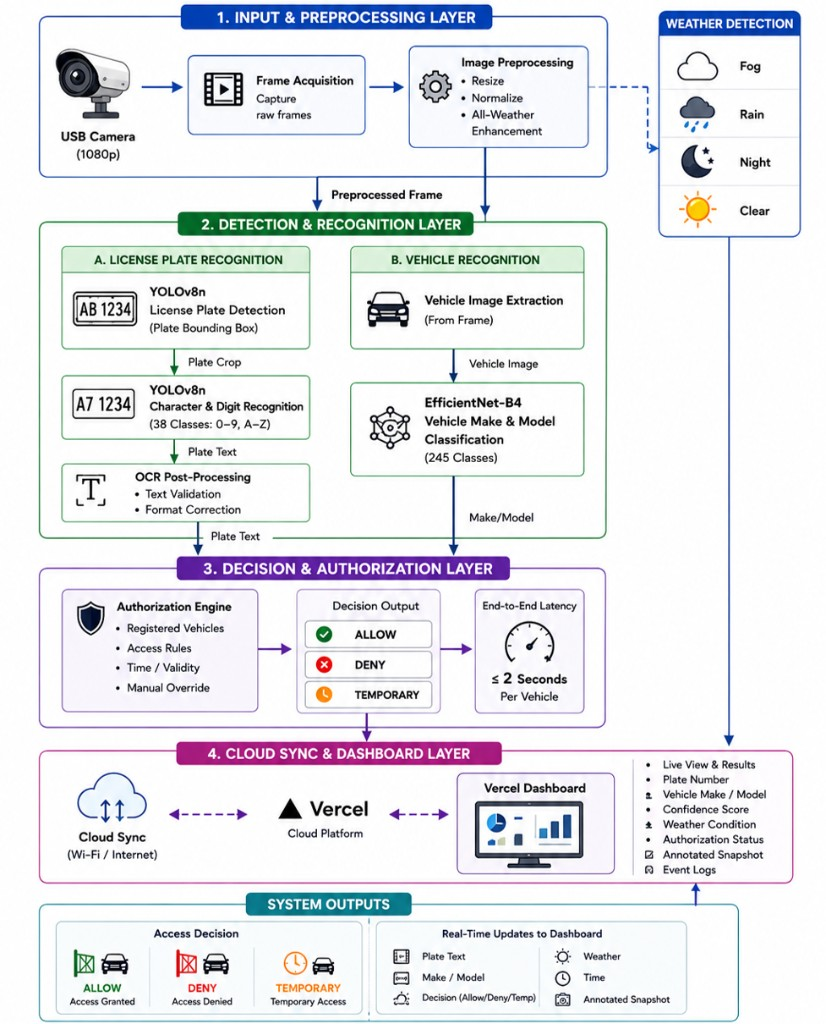
\includegraphics[width=\textwidth,keepaspectratio]{system_overview_diagram.png}
\caption{Overall system architecture of the Automatic Vehicle Gate Access System: camera capture, weather-aware preprocessing, YOLOv8n LPR, EfficientNet-B4 VMMR, dual-modality authorization, and Vercel dashboard sync.}
\label{fig:sys_overview}
\end{figure*}
\FloatBarrier

\begin{figure*}[!htbp]
\centering
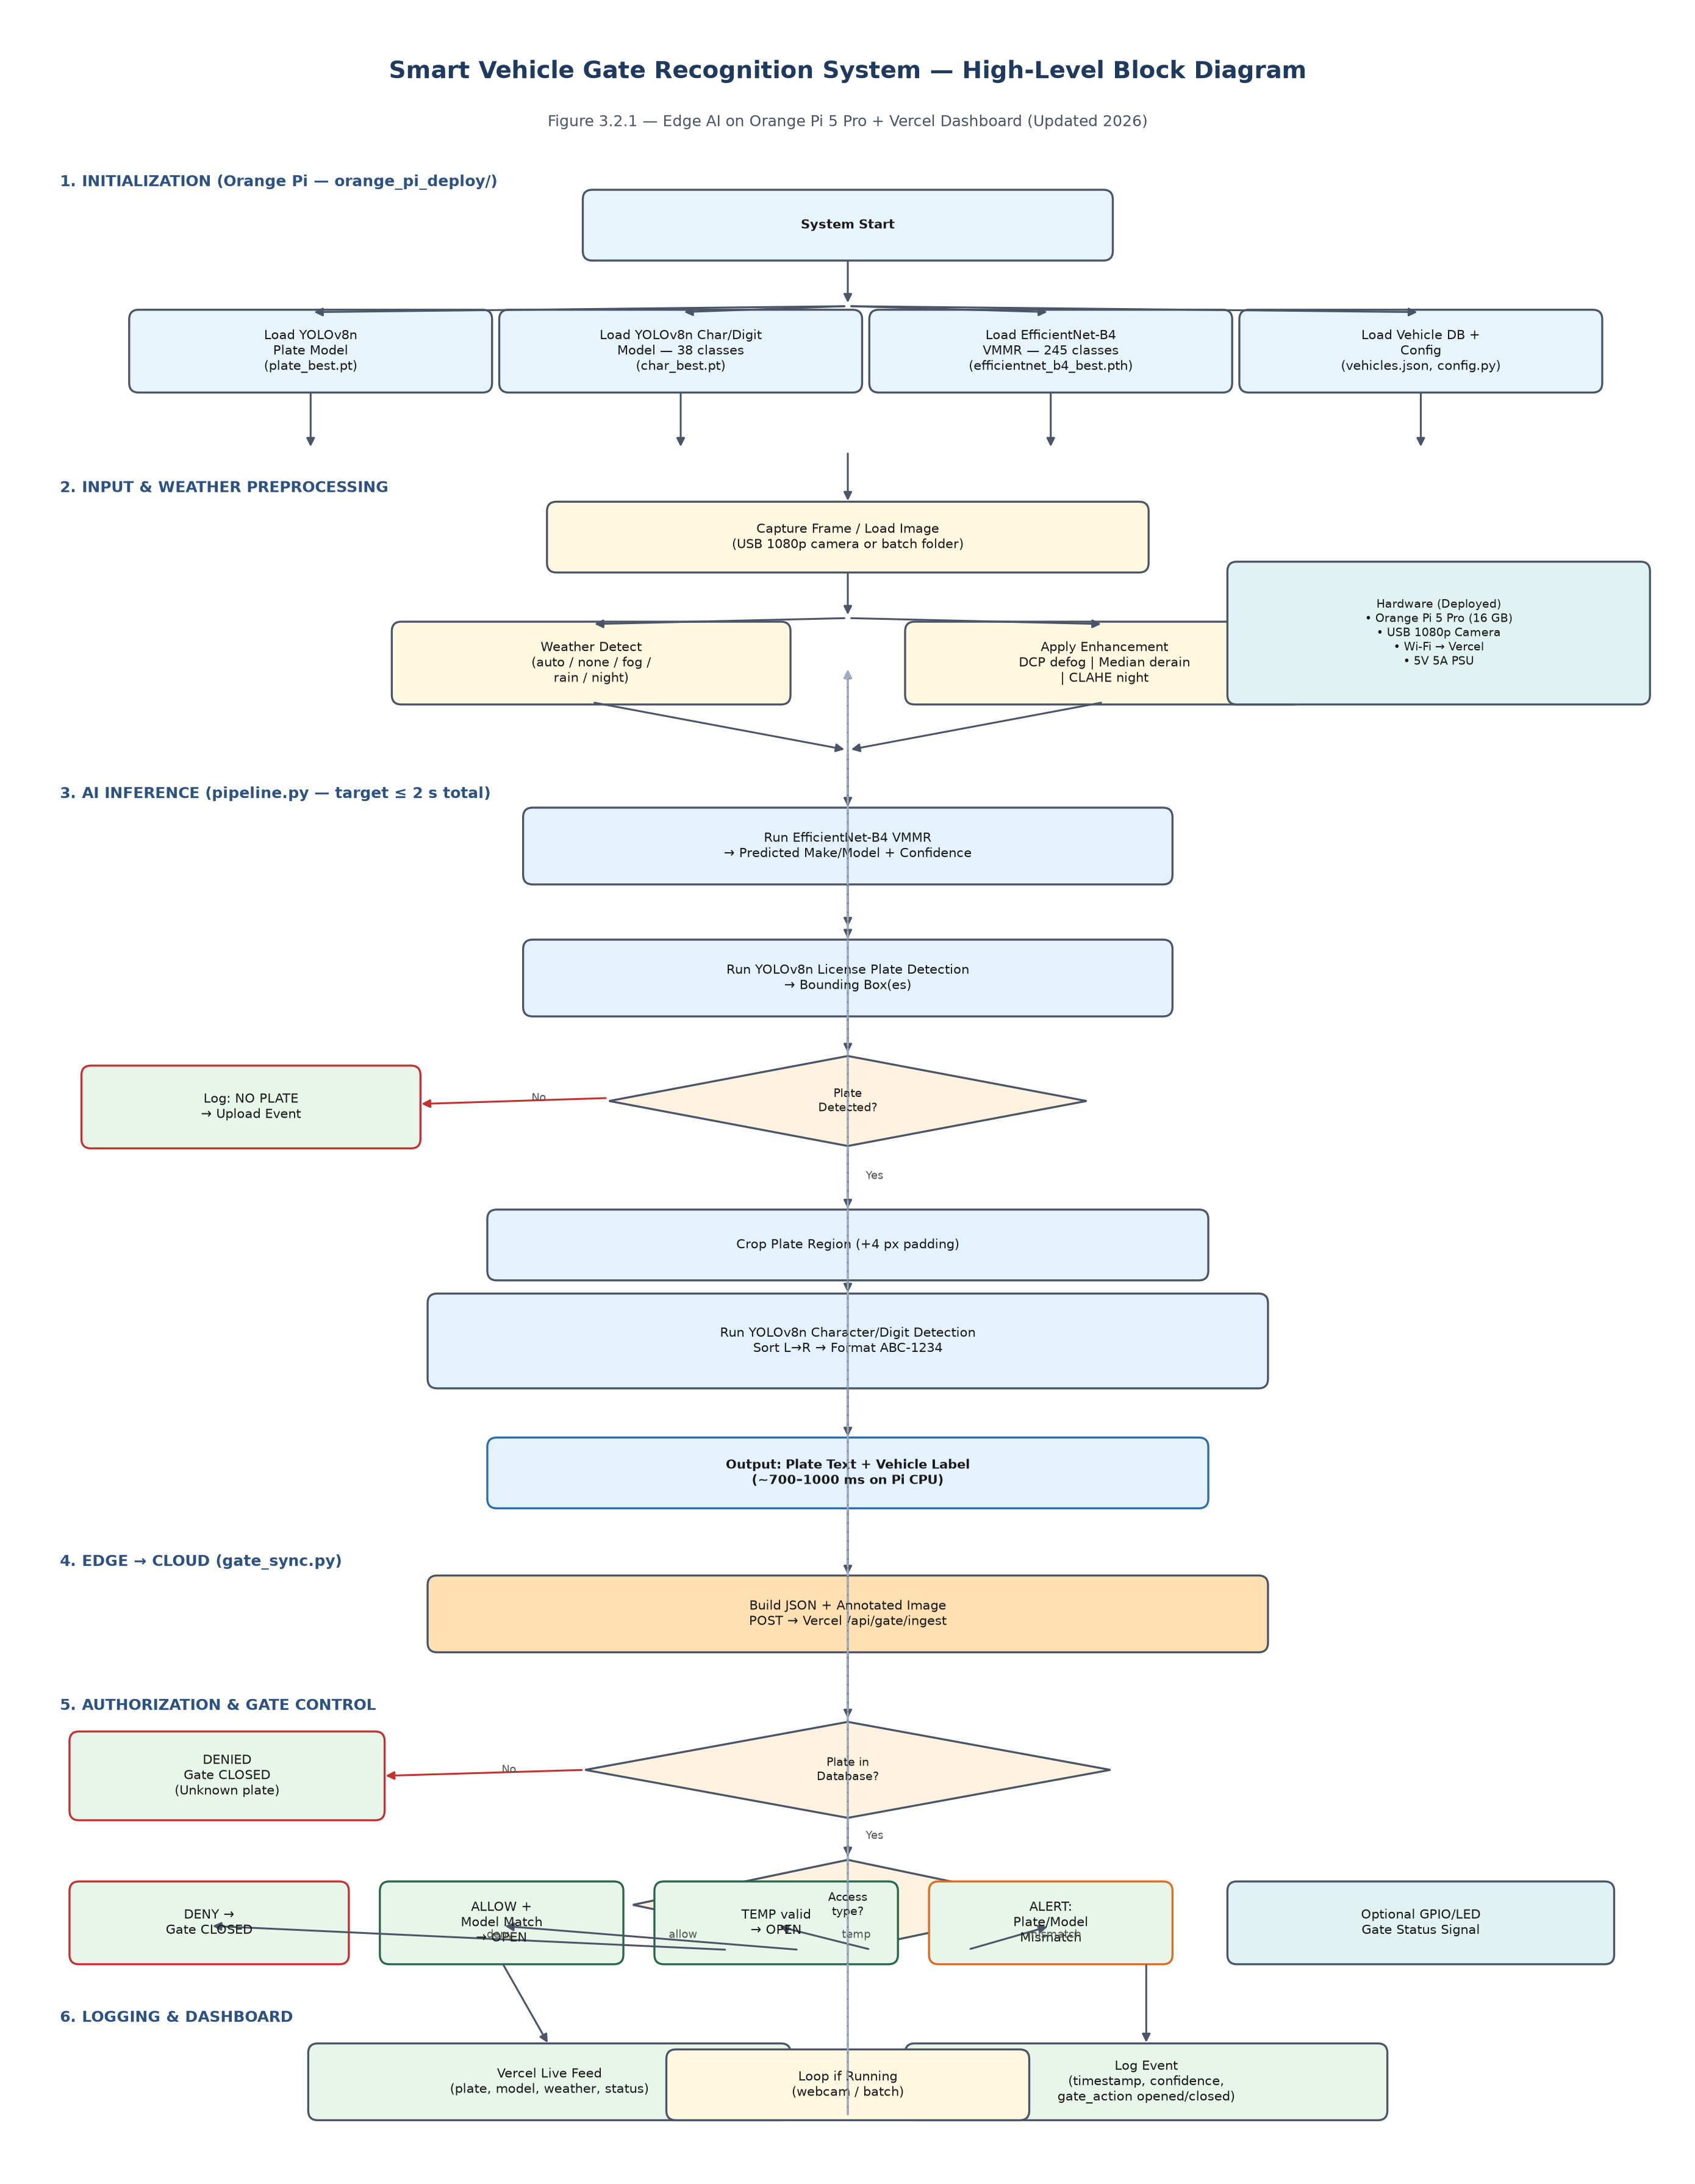
\includegraphics[width=\textwidth,keepaspectratio]{system_block_diagram_updated.png}
\caption{Updated high-level block diagram of the complete FYP pipeline, from Orange Pi model loading through weather branches, AI inference, authorization, and cloud upload.}
\label{fig:sys_block}
\end{figure*}
\FloatBarrier

\begin{figure*}[!htbp]
\centering
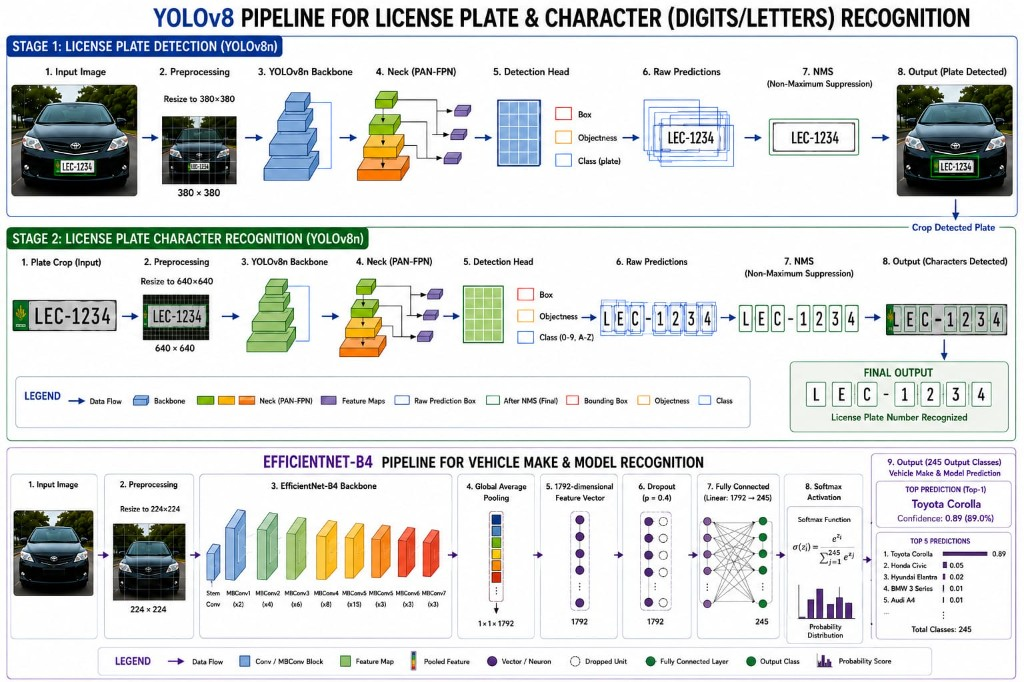
\includegraphics[width=\textwidth,keepaspectratio]{model_architecture_diagram.png}
\caption{Recognition model architectures: two-stage YOLOv8n LPR (plate then 38-class characters) and EfficientNet-B4 VMMR with a 245-way softmax head.}
\label{fig:model_arch}
\end{figure*}
\FloatBarrier

\begin{figure*}[!htbp]
\centering
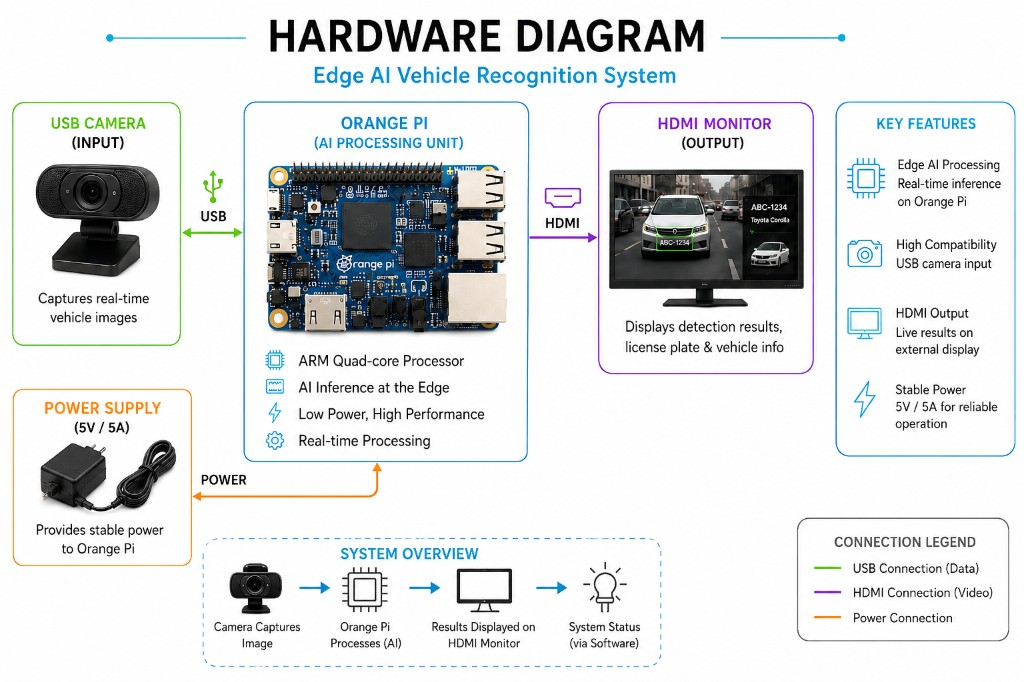
\includegraphics[width=\textwidth,keepaspectratio]{hardware_diagram.png}
\caption{Edge hardware diagram: USB 1080p camera, Orange Pi 5 Pro inference node, HDMI preview, and 5 V/5 A power supply.}
\label{fig:hw_diagram}
\end{figure*}
\FloatBarrier

\begin{figure*}[!htbp]
\centering
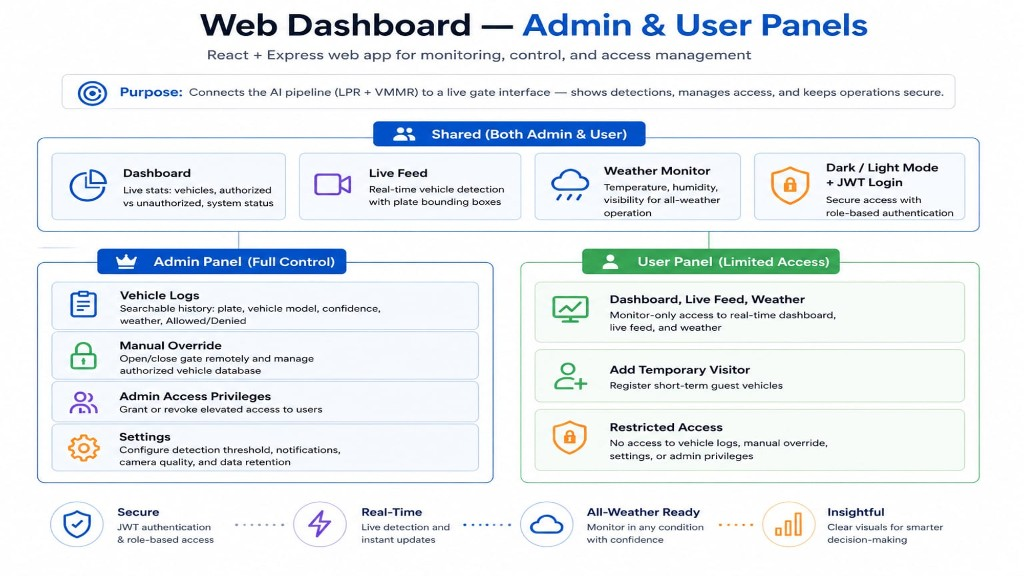
\includegraphics[width=\textwidth,keepaspectratio]{web_dashboard_architecture.png}
\caption{Web dashboard architecture (React front end and Express API on Vercel) with admin versus user roles, live feed, logs, and gate ingest.}
\label{fig:dash_arch}
\end{figure*}
\FloatBarrier

\begin{figure*}[!htbp]
\centering
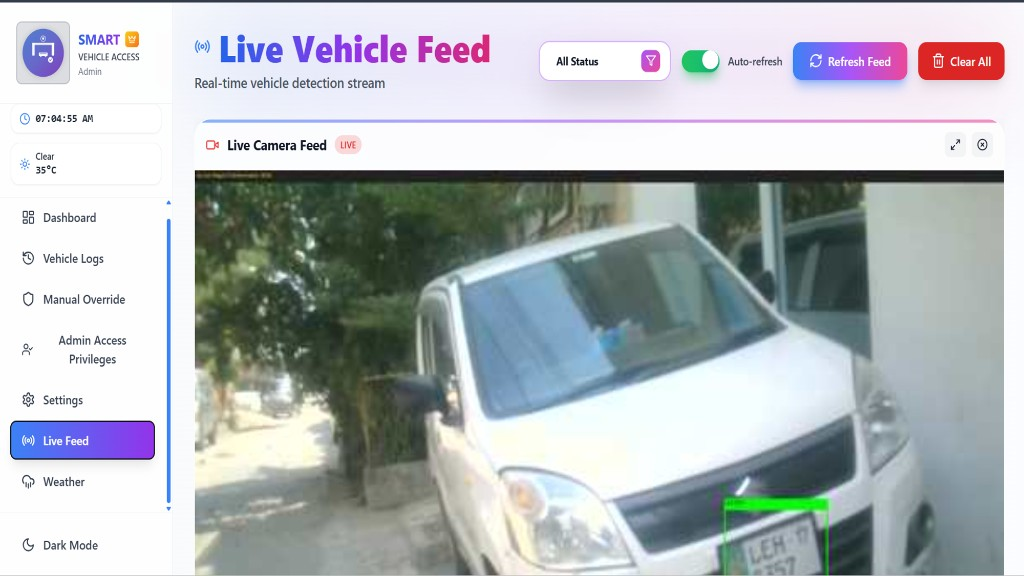
\includegraphics[width=\textwidth,keepaspectratio]{dashboard/admin_live_feed.png}
\caption{Administrator live vehicle feed with full sidebar (logs, manual override, privileges, settings, weather).}
\label{fig:admin_feed}
\end{figure*}
\FloatBarrier

\begin{figure*}[!htbp]
\centering
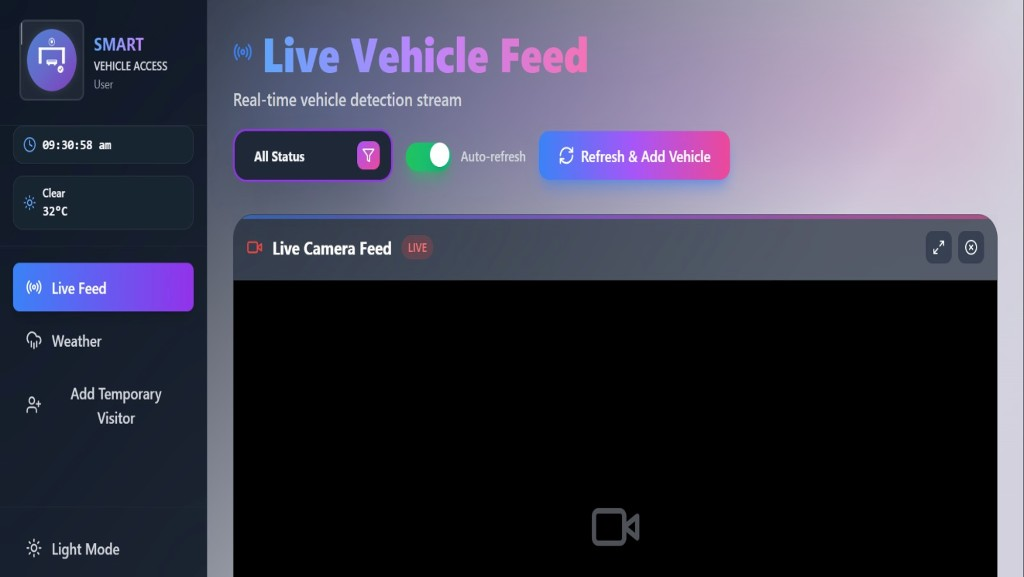
\includegraphics[width=\textwidth,keepaspectratio]{dashboard/user_live_feed.png}
\caption{Standard-user live feed with monitor-only navigation and temporary-visitor registration.}
\label{fig:user_feed}
\end{figure*}
\FloatBarrier

\begin{figure*}[!htbp]
\centering
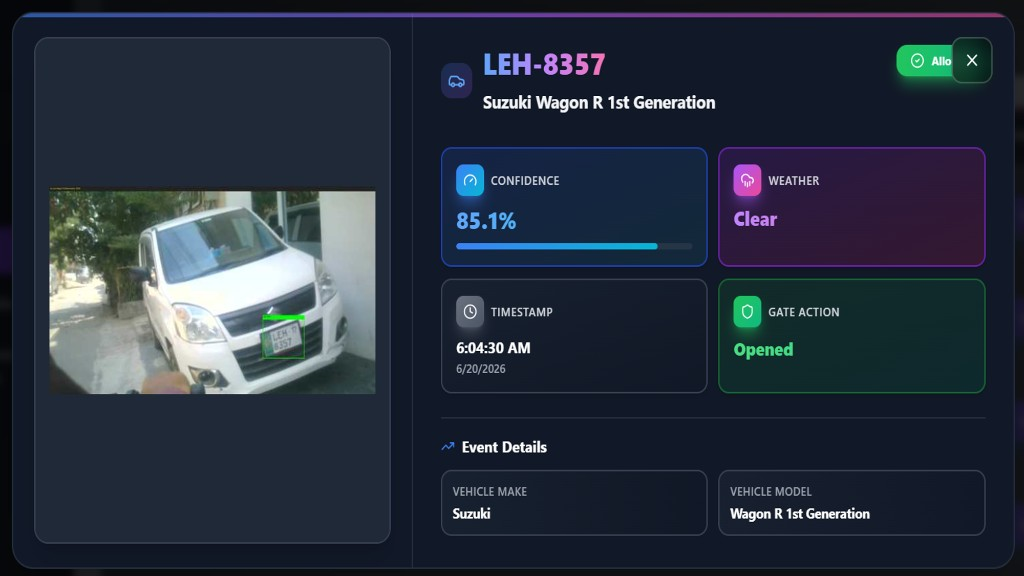
\includegraphics[width=\textwidth,keepaspectratio]{hw/dashboard_allowed.png}
\caption{Dashboard allow event: plate LEH-8357 classified as Suzuki Wagon R and authorized for gate open.}
\label{fig:allow}
\end{figure*}
\FloatBarrier

\begin{figure*}[!htbp]
\centering
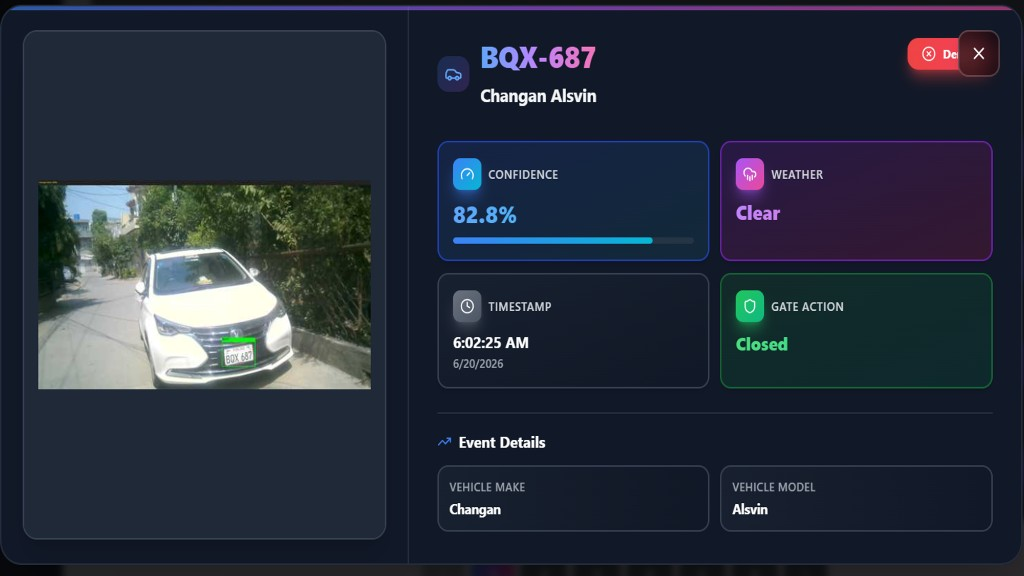
\includegraphics[width=\textwidth,keepaspectratio]{hw/dashboard_denied.png}
\caption{Dashboard deny event: plate BQX-687 (Changan Alsvin) denied when registry/policy checks fail.}
\label{fig:deny}
\end{figure*}
\FloatBarrier

\begin{figure*}[!htbp]
\centering
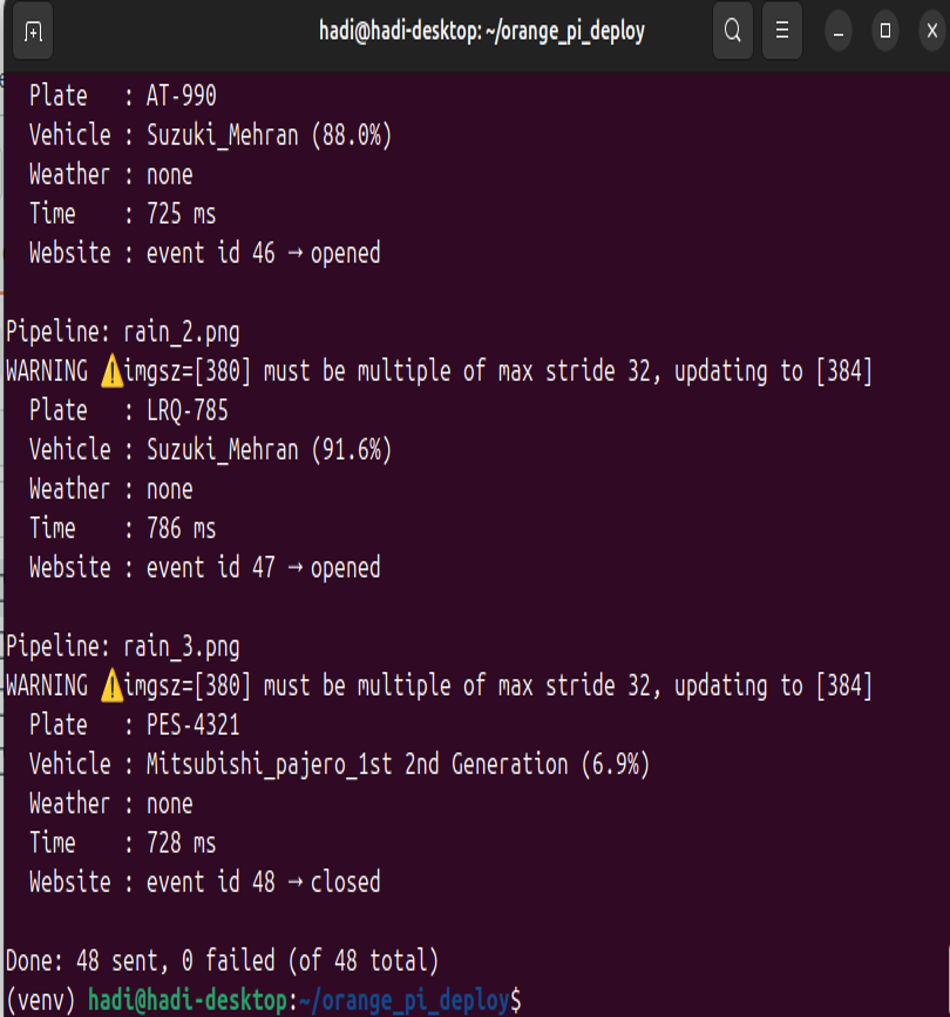
\includegraphics[width=\textwidth,keepaspectratio]{hw/edge_batch_terminal.png}
\caption{Orange Pi batch run over 48 images: plate text, VMMR label, weather branch, latency, and Vercel event IDs.}
\label{fig:edge_batch}
\end{figure*}
\FloatBarrier

\begin{figure*}[!htbp]
\centering
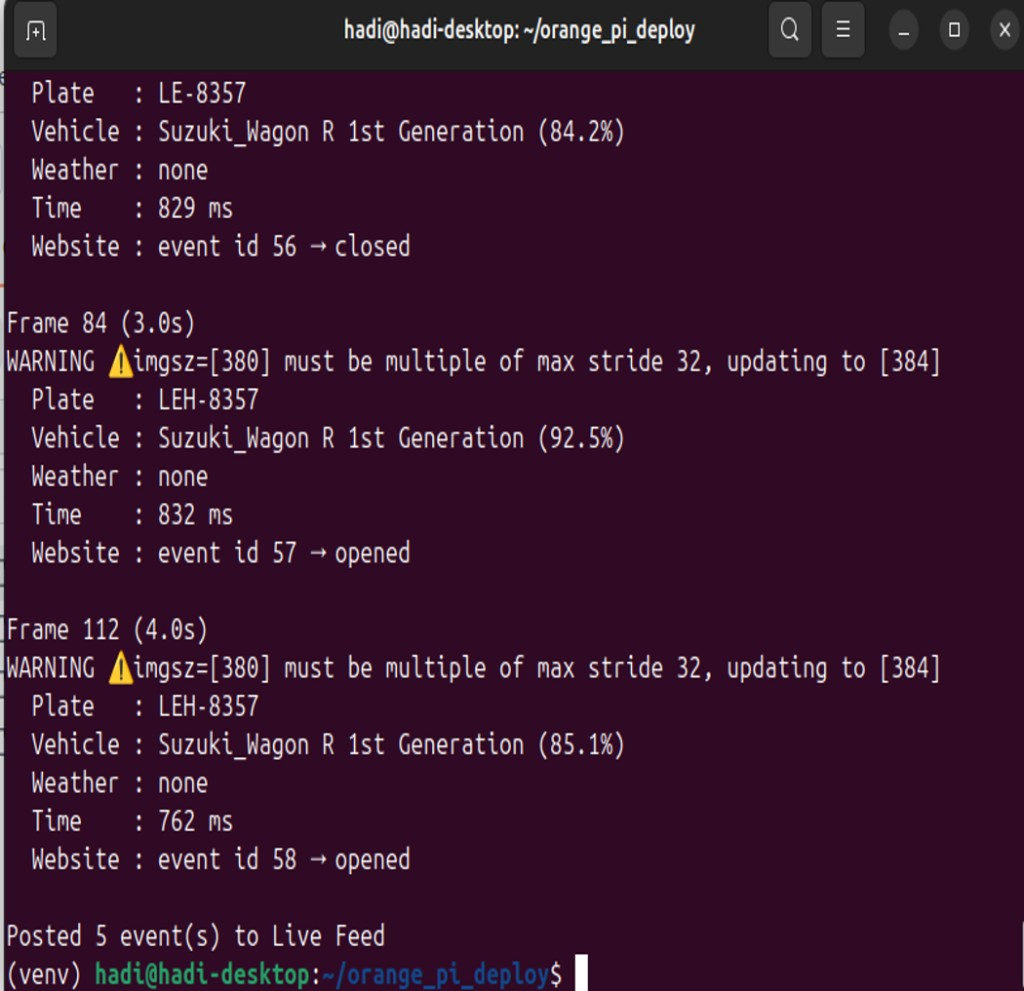
\includegraphics[width=\textwidth,keepaspectratio]{hw/edge_video_terminal.png}
\caption{Real-time video-frame inference on the edge node with plate stabilization and sub-second dashboard POST.}
\label{fig:edge_video}
\end{figure*}
\FloatBarrier

\begin{figure*}[!htbp]
\centering
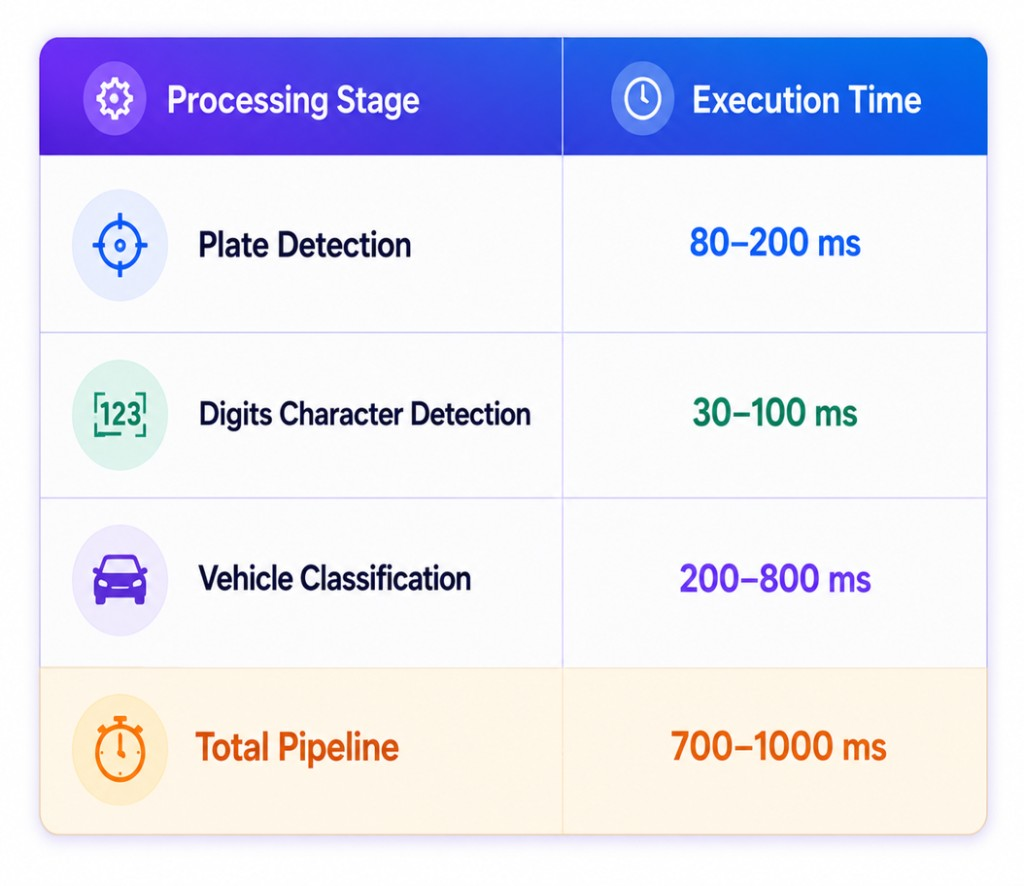
\includegraphics[width=\textwidth,keepaspectratio]{hw/edge_latency_table.png}
\caption{Per-stage edge latency table on Orange Pi 5 Pro CPU (LPD, character OCR, VMMR, and end-to-end).}
\label{fig:edge_lat}
\end{figure*}
\FloatBarrier

\begin{figure*}[!htbp]
\centering
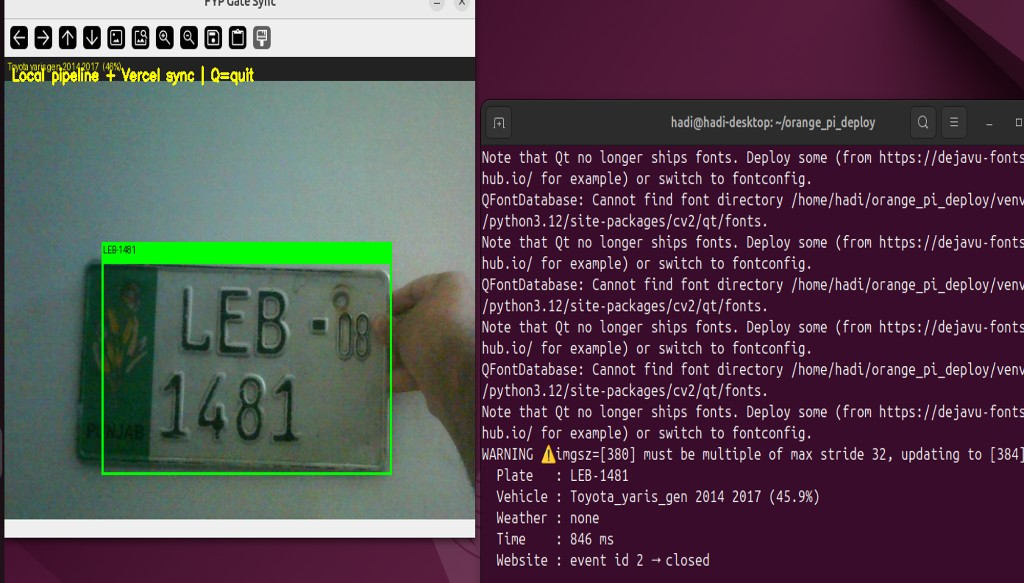
\includegraphics[width=\textwidth,keepaspectratio]{hw/edge_live_gui.png}
\caption{Live Orange Pi GUI demo with plate box overlay and terminal confirming end-to-end inference (~846 ms for LEB-1481).}
\label{fig:edge_gui}
\end{figure*}
\FloatBarrier

\subsection{Weather Preprocessing Figures}
Figures~\ref{fig:pre_fog_in}--\ref{fig:pre_night_out} show fog, rain, and night inputs and restored outputs.

\begin{figure*}[!htbp]
\centering
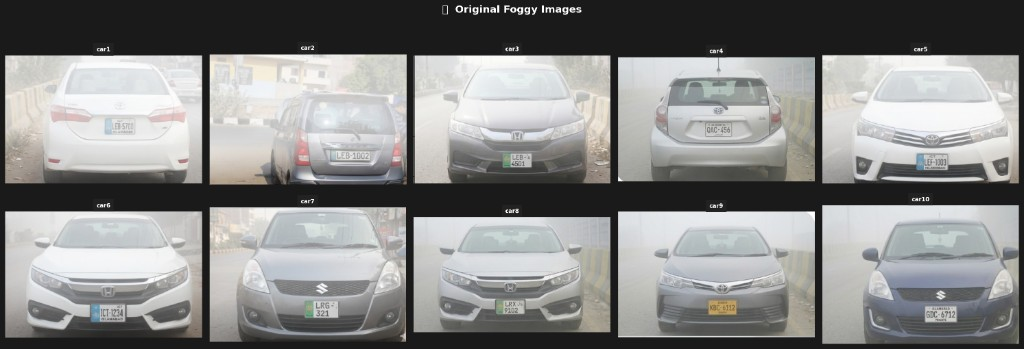
\includegraphics[width=\textwidth,keepaspectratio]{pre/pre_input_foggy.png}
\caption{Original foggy vehicle images before Dark Channel Prior dehazing.}
\label{fig:pre_fog_in}
\end{figure*}
\FloatBarrier

\begin{figure*}[!htbp]
\centering
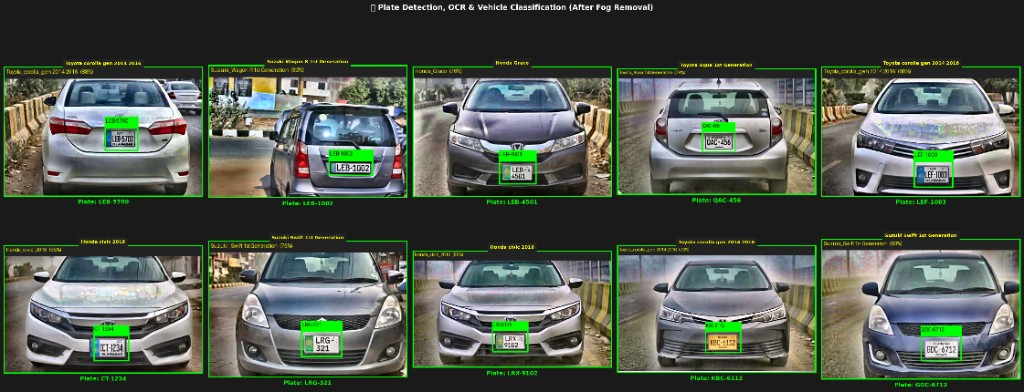
\includegraphics[width=\textwidth,keepaspectratio]{pre/pre_pipeline_defog.png}
\caption{Fog-removal pipeline output after DCP, guided filtering, and contrast restoration.}
\label{fig:pre_fog_out}
\end{figure*}
\FloatBarrier

\begin{figure*}[!htbp]
\centering
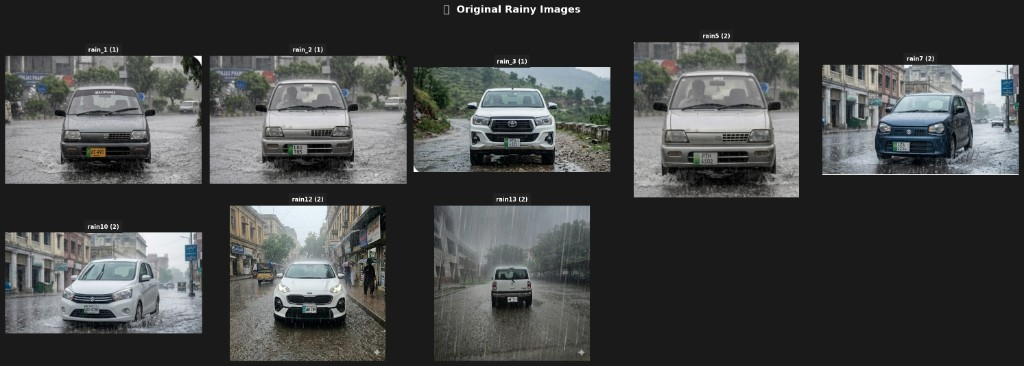
\includegraphics[width=\textwidth,keepaspectratio]{pre/pre_input_rainy.png}
\caption{Original rainy vehicle images showing streaks and glare before rain suppression.}
\label{fig:pre_rain_in}
\end{figure*}
\FloatBarrier

\begin{figure*}[!htbp]
\centering
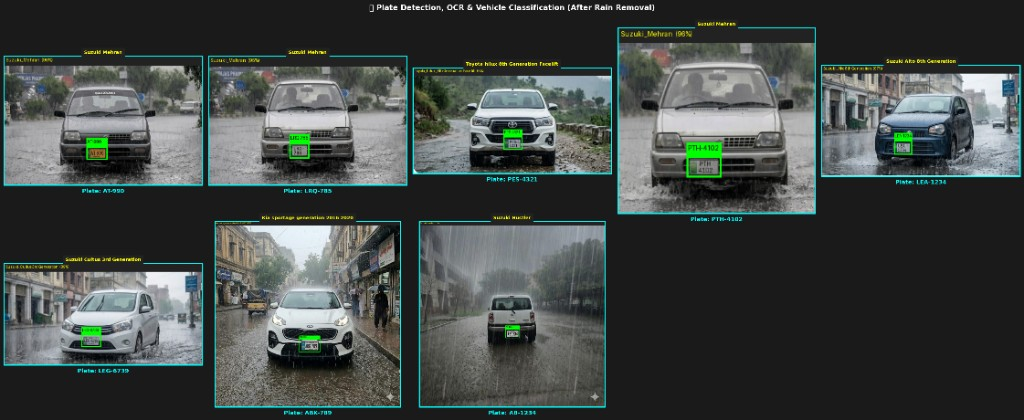
\includegraphics[width=\textwidth,keepaspectratio]{pre/pre_pipeline_rain.png}
\caption{Rain-removal pipeline output after multi-scale vertical median filtering and Telea inpainting.}
\label{fig:pre_rain_out}
\end{figure*}
\FloatBarrier

\begin{figure*}[!htbp]
\centering
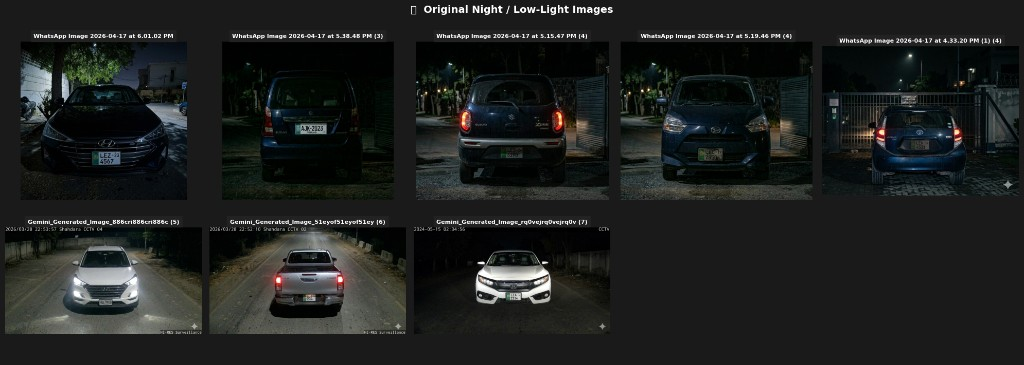
\includegraphics[width=\textwidth,keepaspectratio]{pre/pre_input_night.png}
\caption{Original night / low-light vehicle images before LAB CLAHE enhancement.}
\label{fig:pre_night_in}
\end{figure*}
\FloatBarrier

\begin{figure*}[!htbp]
\centering
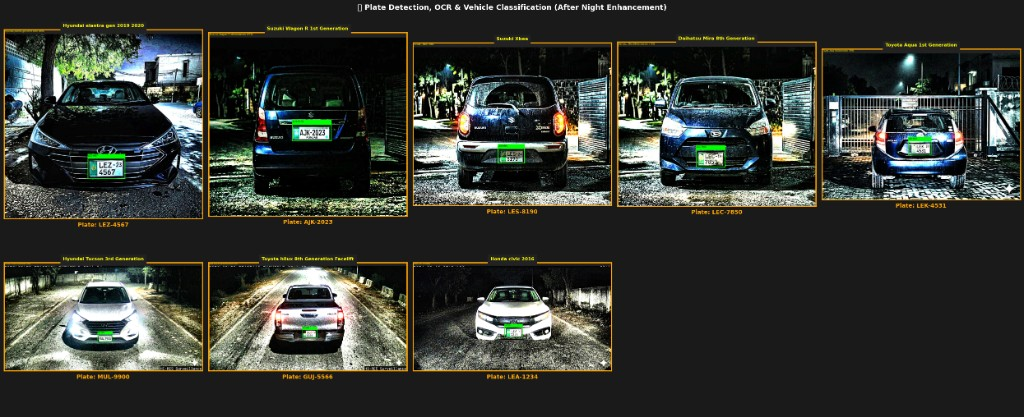
\includegraphics[width=\textwidth,keepaspectratio]{pre/pre_pipeline_night.png}
\caption{Night-enhancement pipeline output after LAB CLAHE, gamma correction, and edge recovery.}
\label{fig:pre_night_out}
\end{figure*}
\FloatBarrier

\subsection{License Plate Detection Figures}
Figures~\ref{fig:lpd_labels}--\ref{fig:lpd_hwy} cover dataset diagnostics, 50-epoch training curves, PR/F1 curves, confusion matrices, and qualitative detections. Epoch-50 validation metrics are precision 98.50\%, recall 95.53\%, and mAP@0.5 98.07\%.

\begin{figure*}[!htbp]
\centering
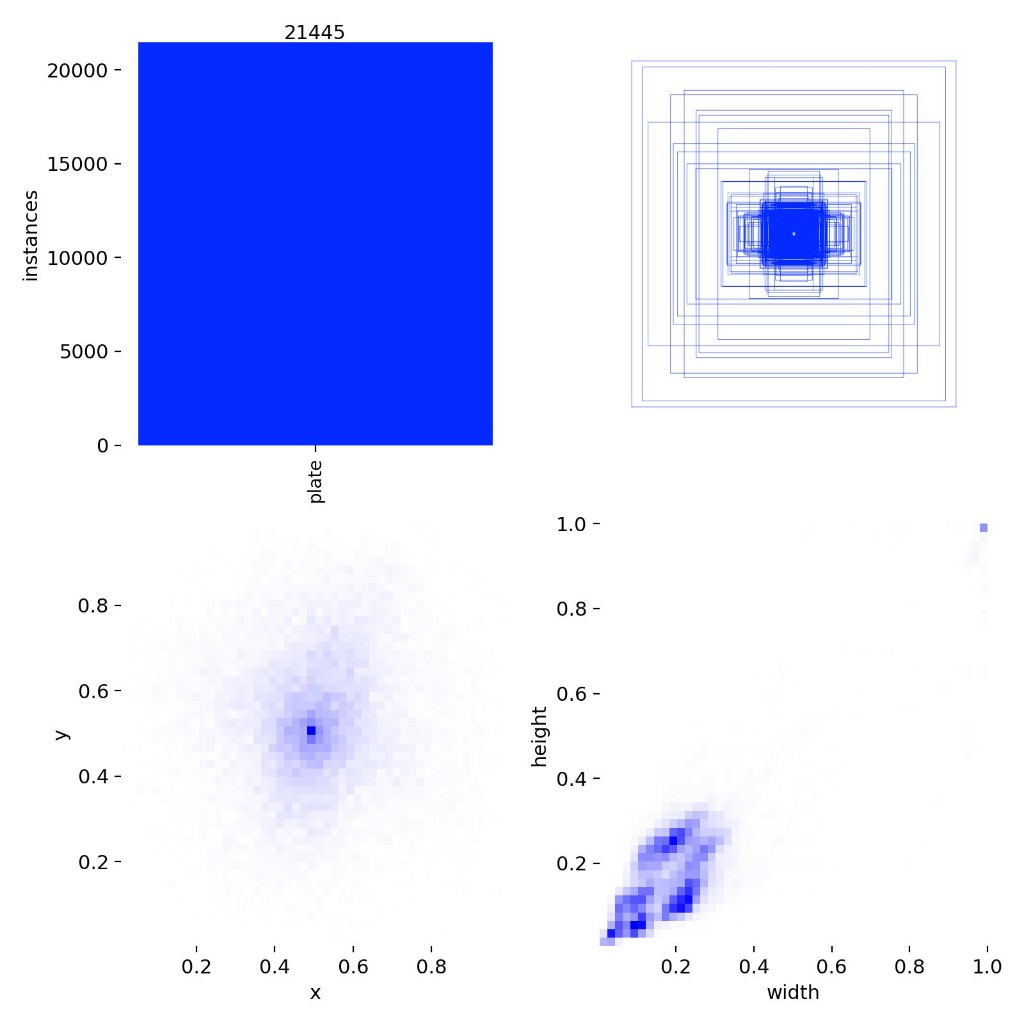
\includegraphics[width=\textwidth,keepaspectratio]{lpd/lpd_dataset_labels.png}
\caption{License-plate detection dataset label analysis: class counts, box shapes, and spatial distributions.}
\label{fig:lpd_labels}
\end{figure*}
\FloatBarrier

\begin{figure*}[!htbp]
\centering
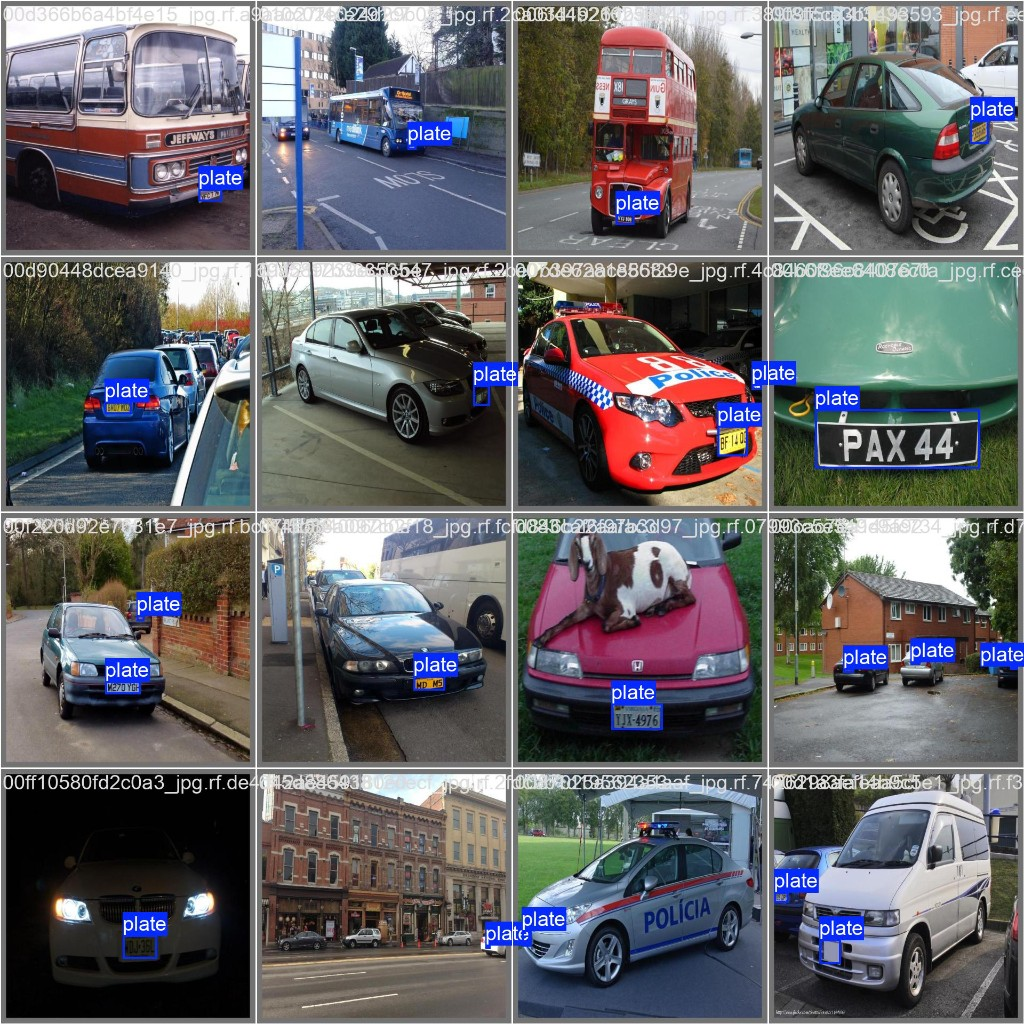
\includegraphics[width=\textwidth,keepaspectratio]{lpd/lpd_val_batch_labels.png}
\caption{LPD validation batch mosaic with ground-truth plate boxes on Roboflow-style tiles.}
\label{fig:lpd_valbatch}
\end{figure*}
\FloatBarrier

\begin{figure*}[!htbp]
\centering
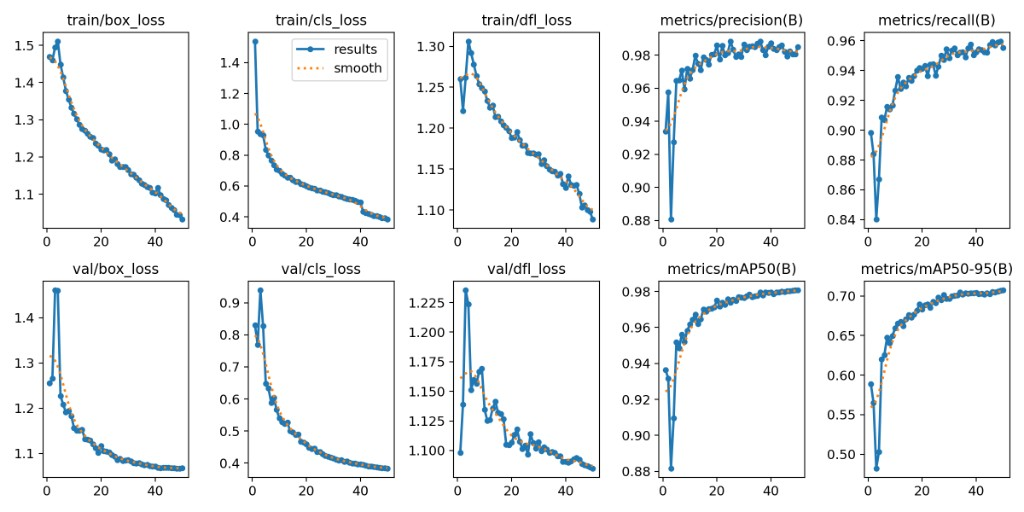
\includegraphics[width=\textwidth,keepaspectratio]{lpd/lpd_training_results.png}
\caption{YOLOv8n LPD training curves over 50 epochs (loss, precision, recall, mAP@0.5, mAP@0.5:0.95).}
\label{fig:lpd_train}
\end{figure*}
\FloatBarrier

\begin{figure*}[!htbp]
\centering
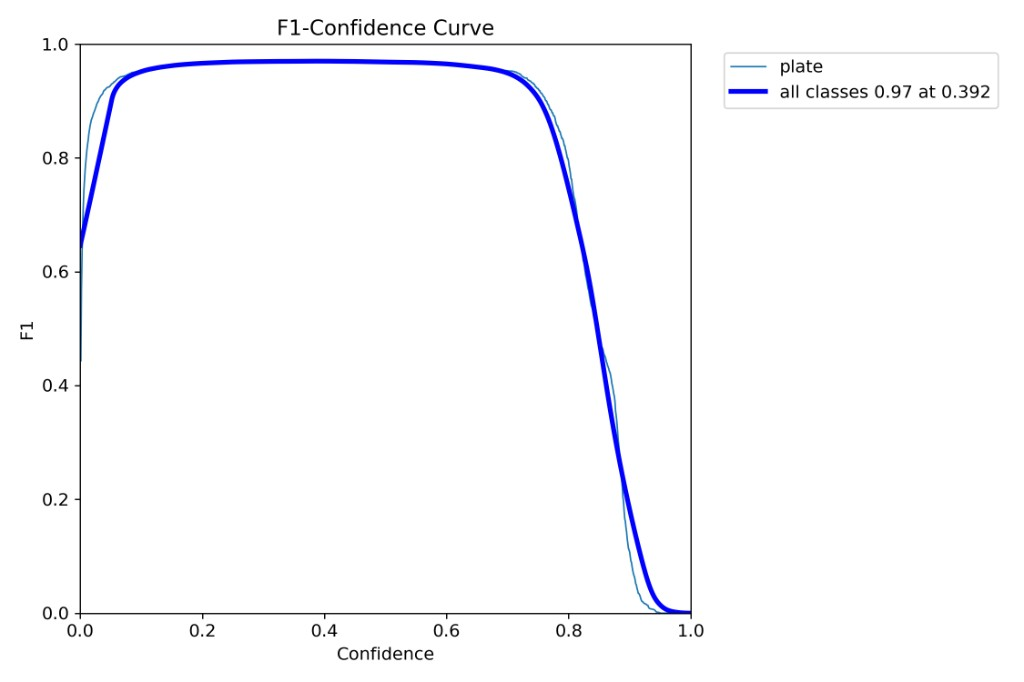
\includegraphics[width=\textwidth,keepaspectratio]{lpd/lpd_curve_f1.png}
\caption{LPD F1--confidence curve for the plate class.}
\label{fig:lpd_f1}
\end{figure*}
\FloatBarrier

\begin{figure*}[!htbp]
\centering
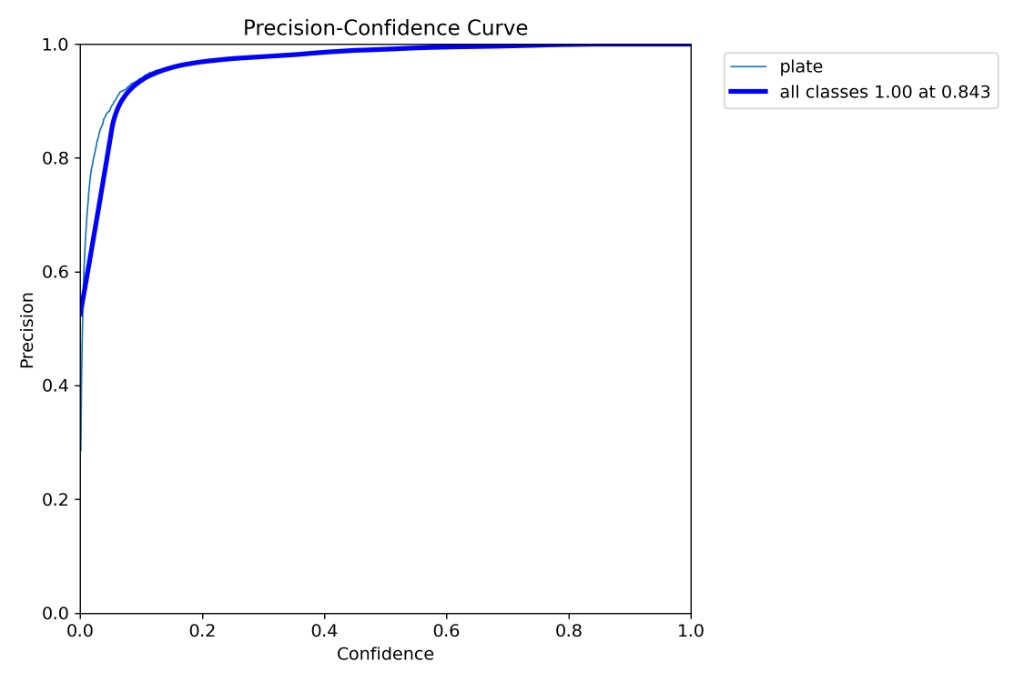
\includegraphics[width=\textwidth,keepaspectratio]{lpd/lpd_curve_precision.png}
\caption{LPD precision--confidence curve for the plate class.}
\label{fig:lpd_p}
\end{figure*}
\FloatBarrier

\begin{figure*}[!htbp]
\centering
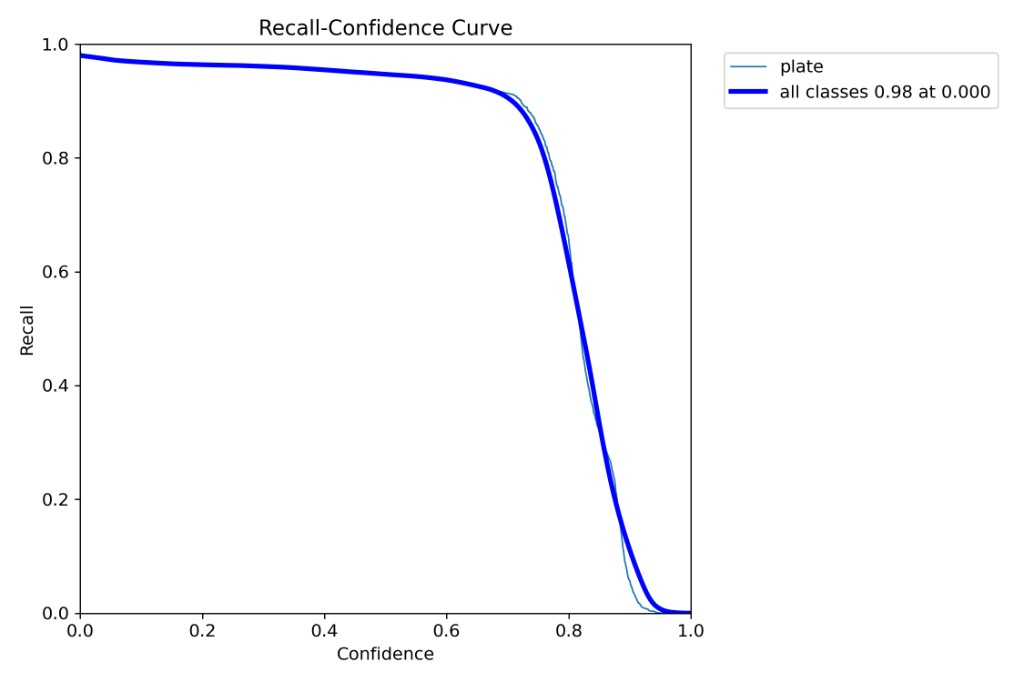
\includegraphics[width=\textwidth,keepaspectratio]{lpd/lpd_curve_recall.png}
\caption{LPD recall--confidence curve for the plate class.}
\label{fig:lpd_r}
\end{figure*}
\FloatBarrier

\begin{figure*}[!htbp]
\centering
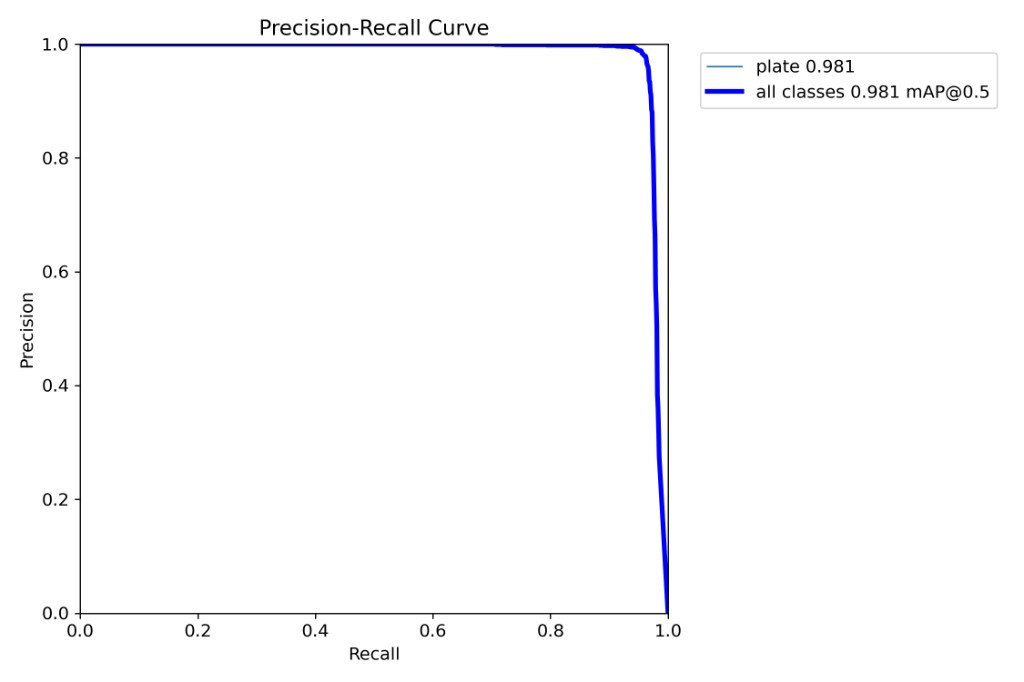
\includegraphics[width=\textwidth,keepaspectratio]{lpd/lpd_curve_pr.png}
\caption{LPD precision--recall curve (mAP@0.5).}
\label{fig:lpd_pr}
\end{figure*}
\FloatBarrier

\begin{figure*}[!htbp]
\centering
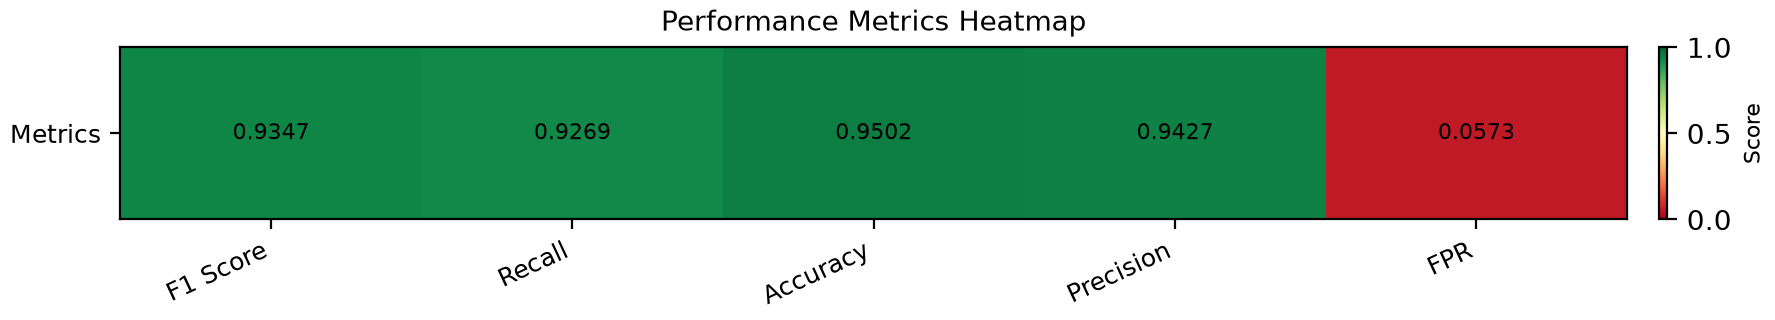
\includegraphics[width=\textwidth,keepaspectratio]{lpd/lpd_metrics_heatmap.png}
\caption{LPD diagnostic metrics heatmap from the validation export.}
\label{fig:lpd_heat}
\end{figure*}
\FloatBarrier

\begin{figure*}[!htbp]
\centering
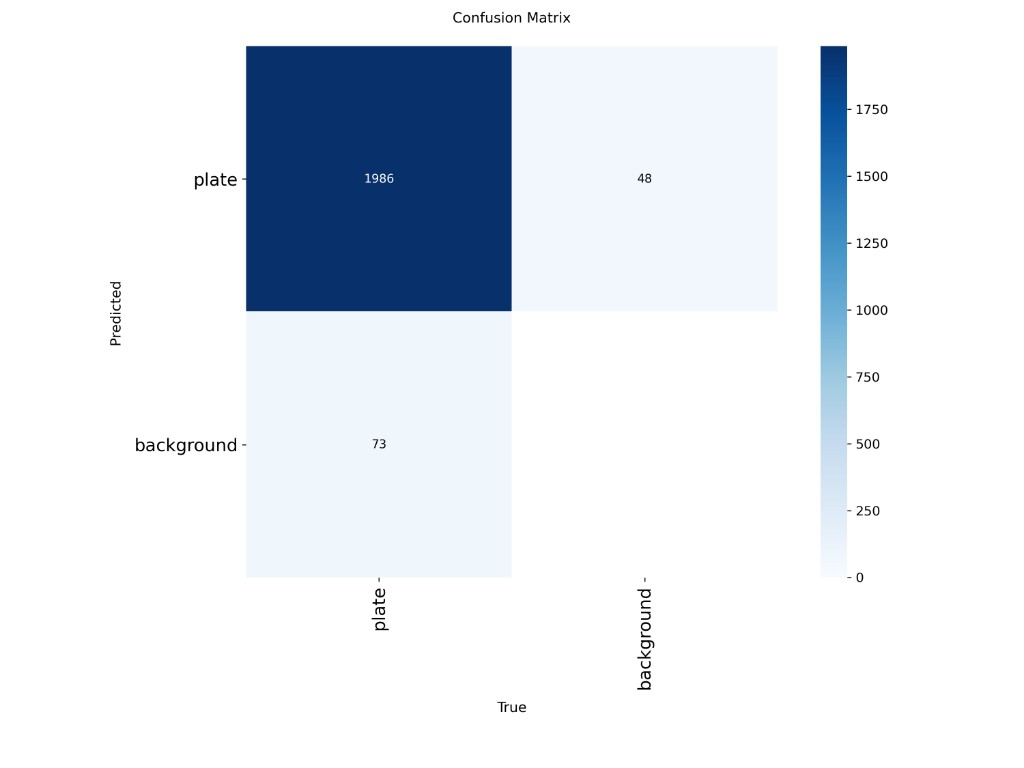
\includegraphics[width=\textwidth,keepaspectratio]{lpd/lpd_confusion_matrix.png}
\caption{LPD confusion matrix (counts) for plate versus background.}
\label{fig:lpd_cm}
\end{figure*}
\FloatBarrier

\begin{figure*}[!htbp]
\centering
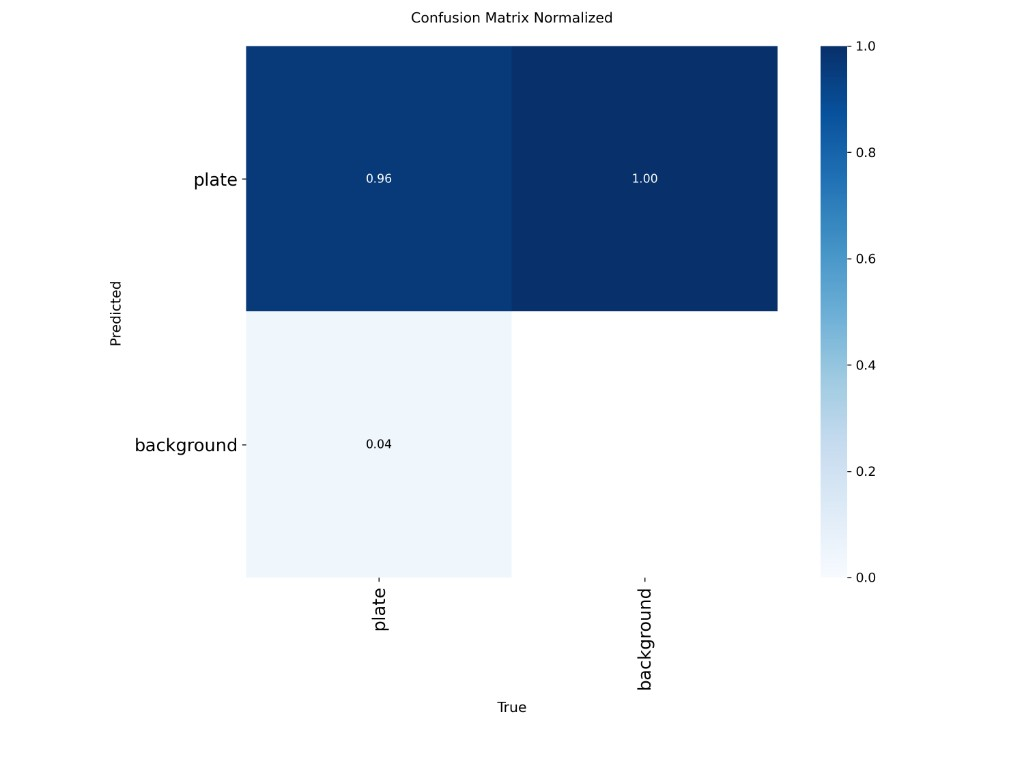
\includegraphics[width=\textwidth,keepaspectratio]{lpd/lpd_confusion_normalized.png}
\caption{LPD row-normalized confusion matrix for plate versus background.}
\label{fig:lpd_cmn}
\end{figure*}
\FloatBarrier

\begin{figure*}[!htbp]
\centering
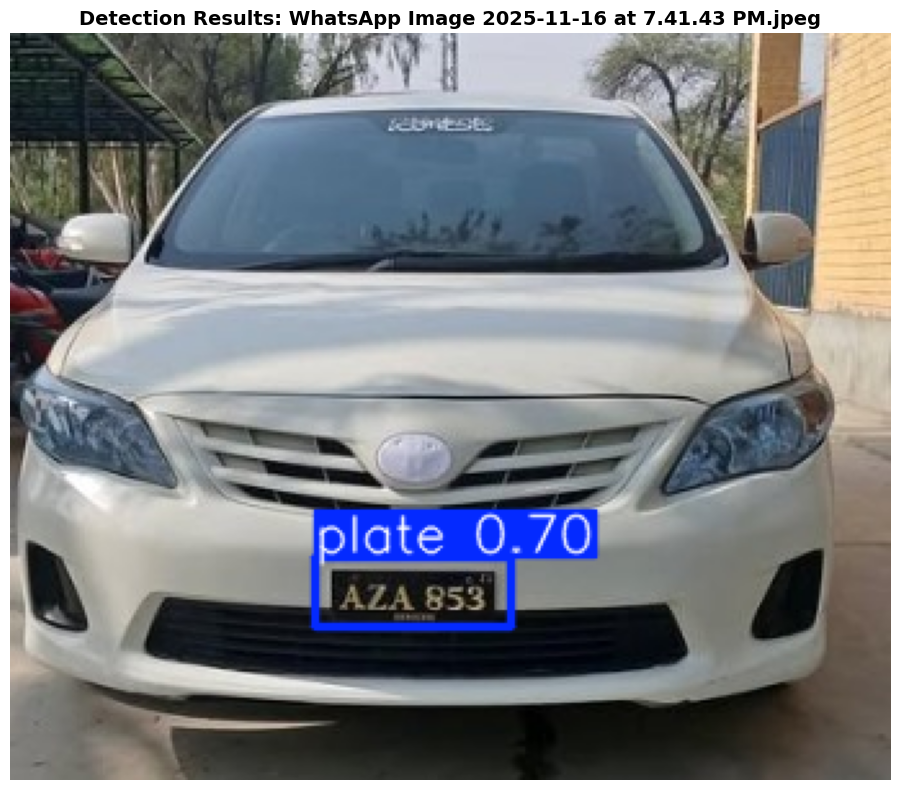
\includegraphics[width=\textwidth,keepaspectratio]{lpd/lpd_pred_clear_corolla.png}
\caption{Qualitative LPD result: clear daylight frontal sedan with plate box and confidence.}
\label{fig:lpd_corolla}
\end{figure*}
\FloatBarrier

\begin{figure*}[!htbp]
\centering
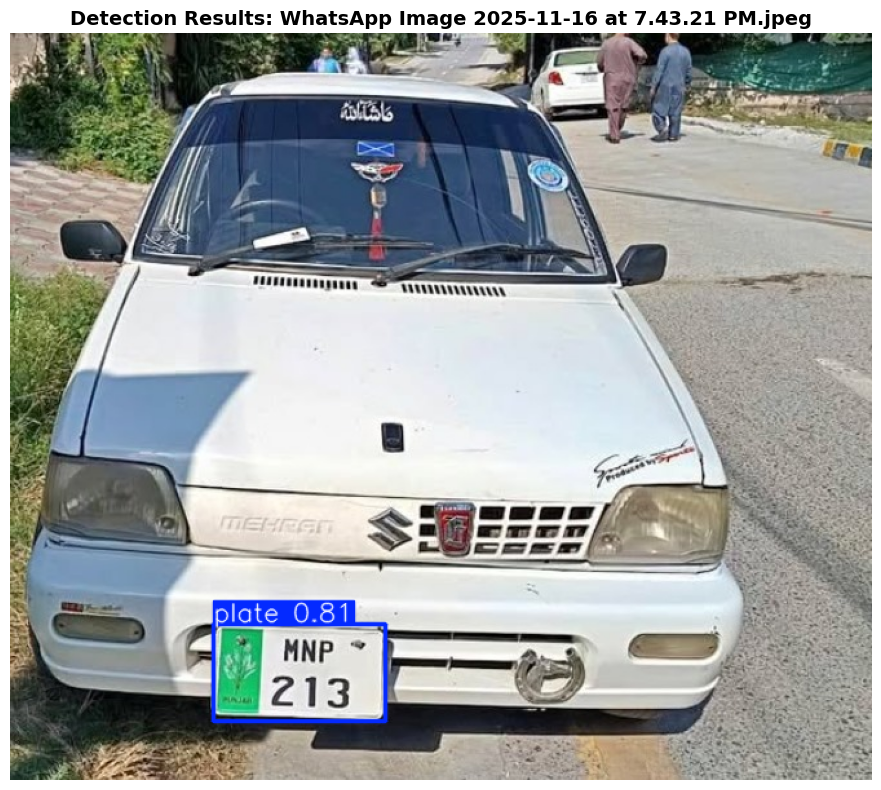
\includegraphics[width=\textwidth,keepaspectratio]{lpd/lpd_pred_clear_mehran.png}
\caption{Qualitative LPD result: clear daylight regional plate styling.}
\label{fig:lpd_mehran}
\end{figure*}
\FloatBarrier

\begin{figure*}[!htbp]
\centering
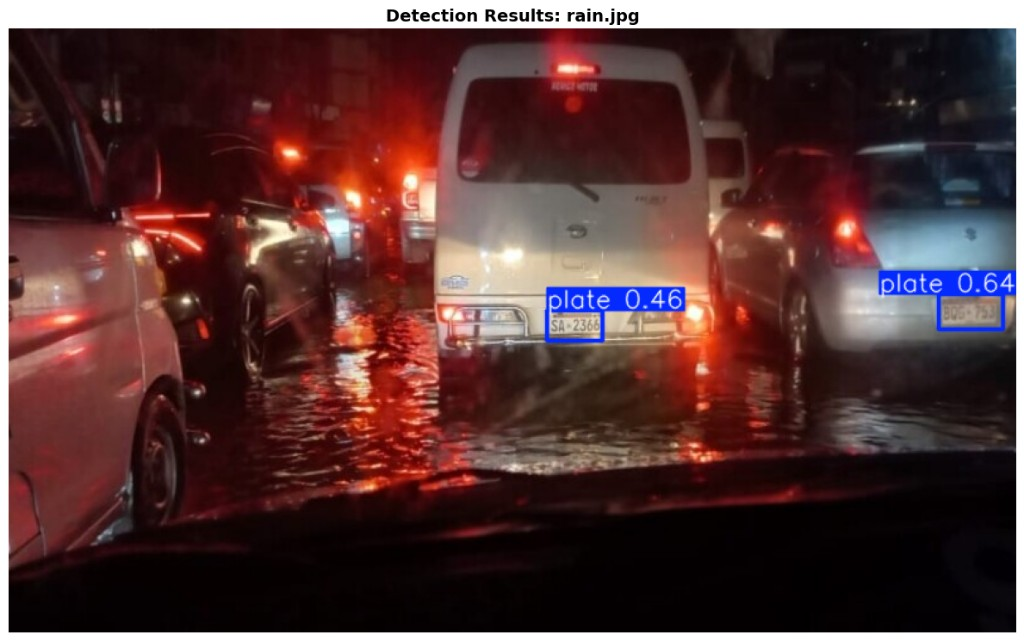
\includegraphics[width=\textwidth,keepaspectratio]{lpd/lpd_pred_rain_night.png}
\caption{Qualitative LPD result: rain/night scene with glare and plate detections.}
\label{fig:lpd_rain}
\end{figure*}
\FloatBarrier

\begin{figure*}[!htbp]
\centering
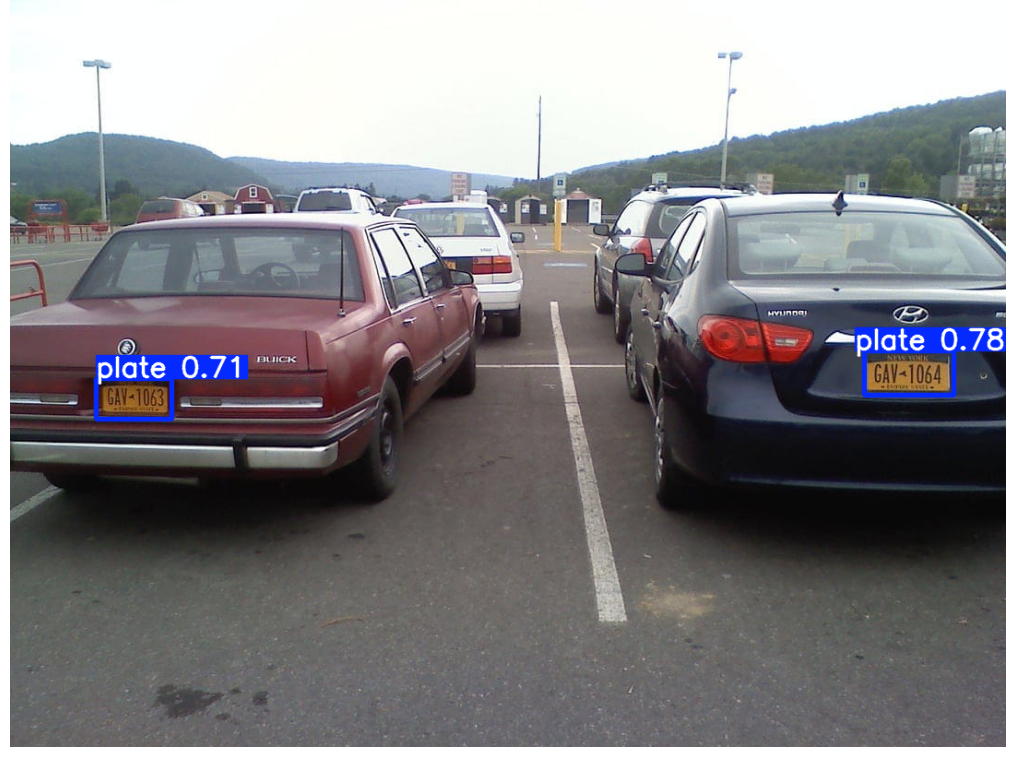
\includegraphics[width=\textwidth,keepaspectratio]{lpd/lpd_pred_parking_dual.png}
\caption{Qualitative LPD result: parking-lot scene with dual plate detections.}
\label{fig:lpd_park}
\end{figure*}
\FloatBarrier

\begin{figure*}[!htbp]
\centering
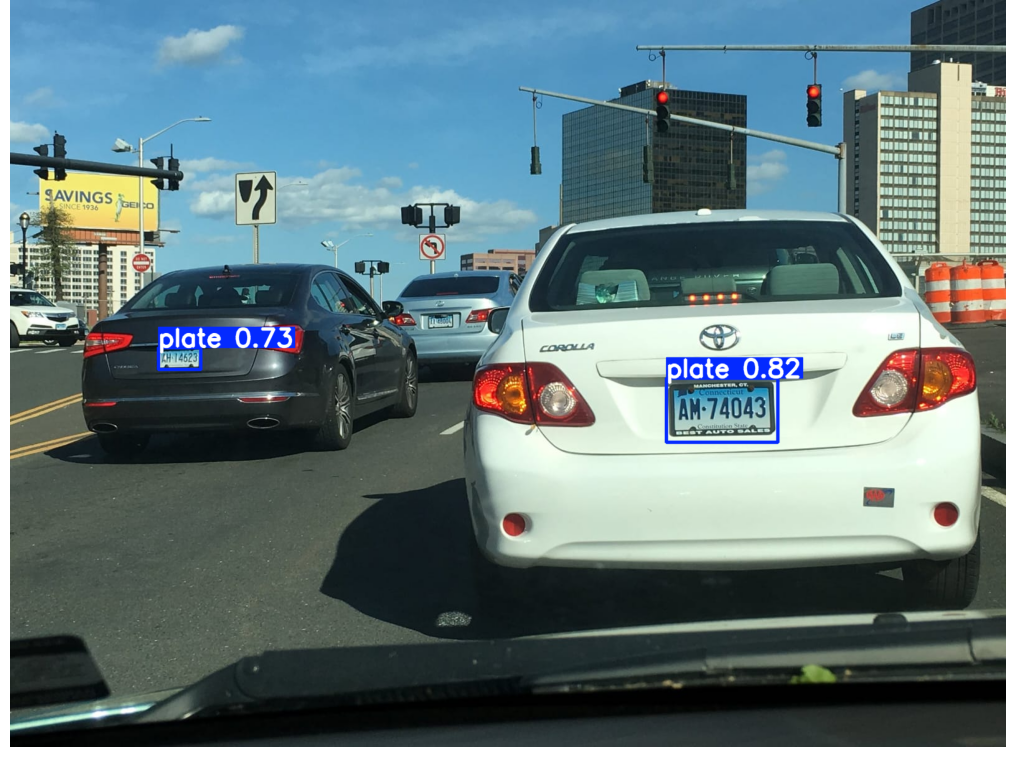
\includegraphics[width=\textwidth,keepaspectratio]{lpd/lpd_pred_highway_dual.png}
\caption{Qualitative LPD result: highway multi-lane scene with distant plates.}
\label{fig:lpd_hwy}
\end{figure*}
\FloatBarrier

\subsection{Character Recognition Figures}
Figures~\ref{fig:ocr_labels}--\ref{fig:ocr_e2e} cover the 38-class detector. Canonical project metrics are mAP@0.5 97.7\%, precision 99.0\%, recall 94.2\%, and F1 96.5\% under mirrored validation.

\begin{figure*}[!htbp]
\centering
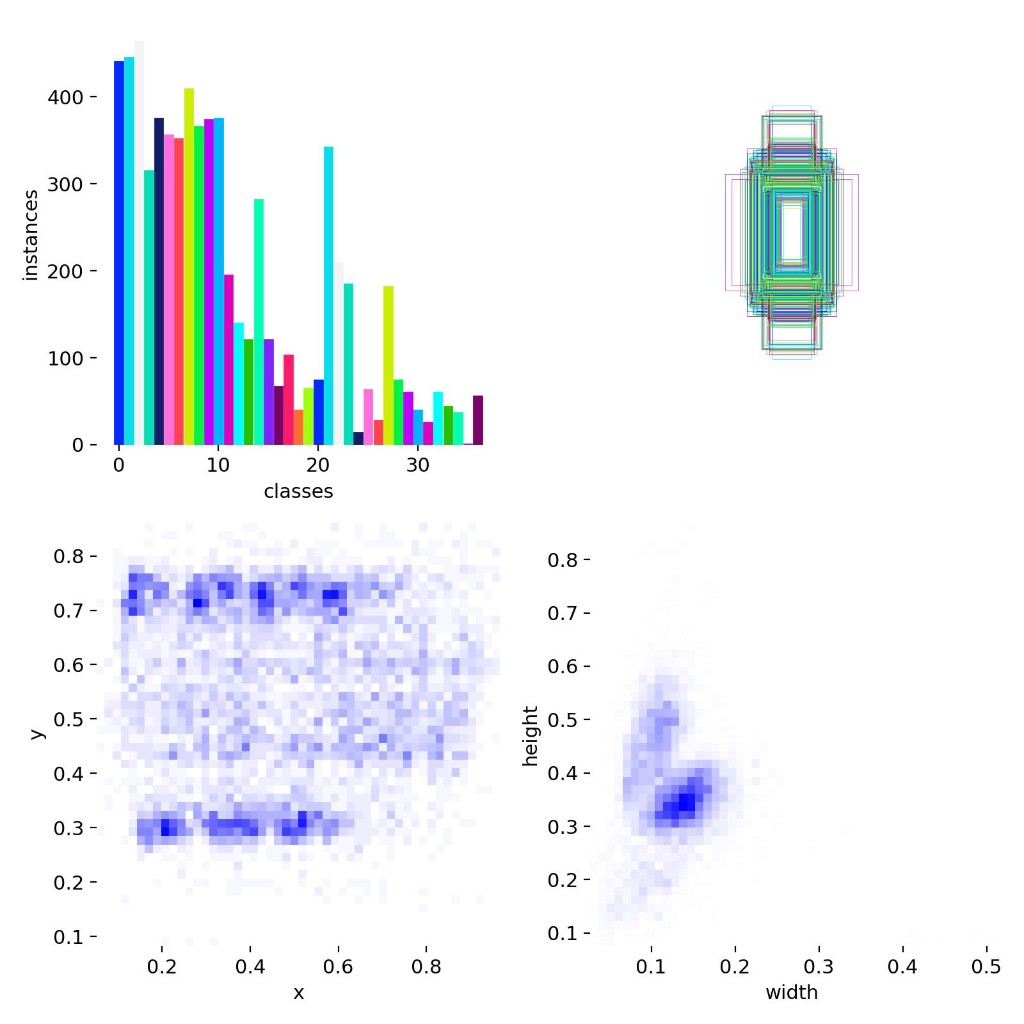
\includegraphics[width=\textwidth,keepaspectratio]{lpr_char/ocr_labels.png}
\caption{Character-recognition dataset label distribution across 38 alphanumeric classes.}
\label{fig:ocr_labels}
\end{figure*}
\FloatBarrier

\begin{figure*}[!htbp]
\centering
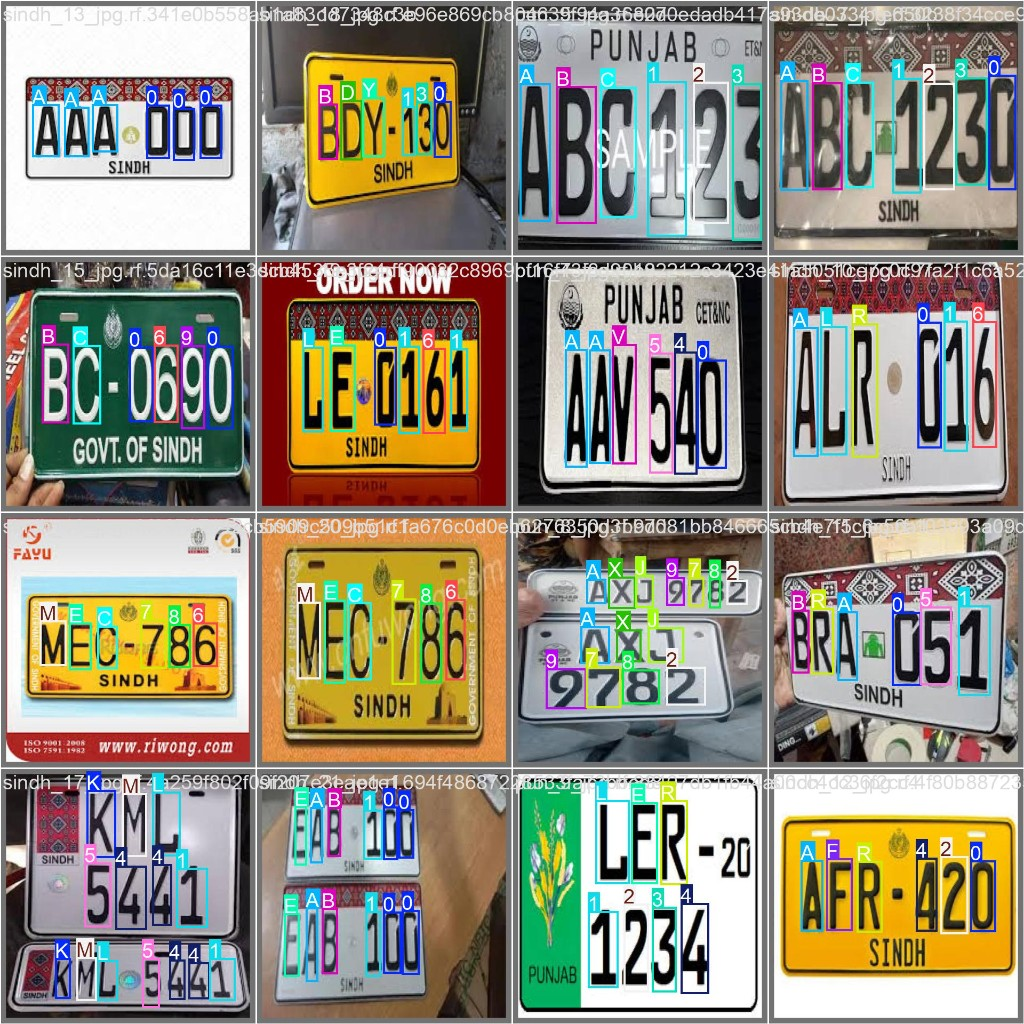
\includegraphics[width=\textwidth,keepaspectratio]{lpr_char/ocr_val_batch0_labels.png}
\caption{Character validation batch mosaic (batch 0) with ground-truth glyph boxes.}
\label{fig:ocr_val0}
\end{figure*}
\FloatBarrier

\begin{figure*}[!htbp]
\centering
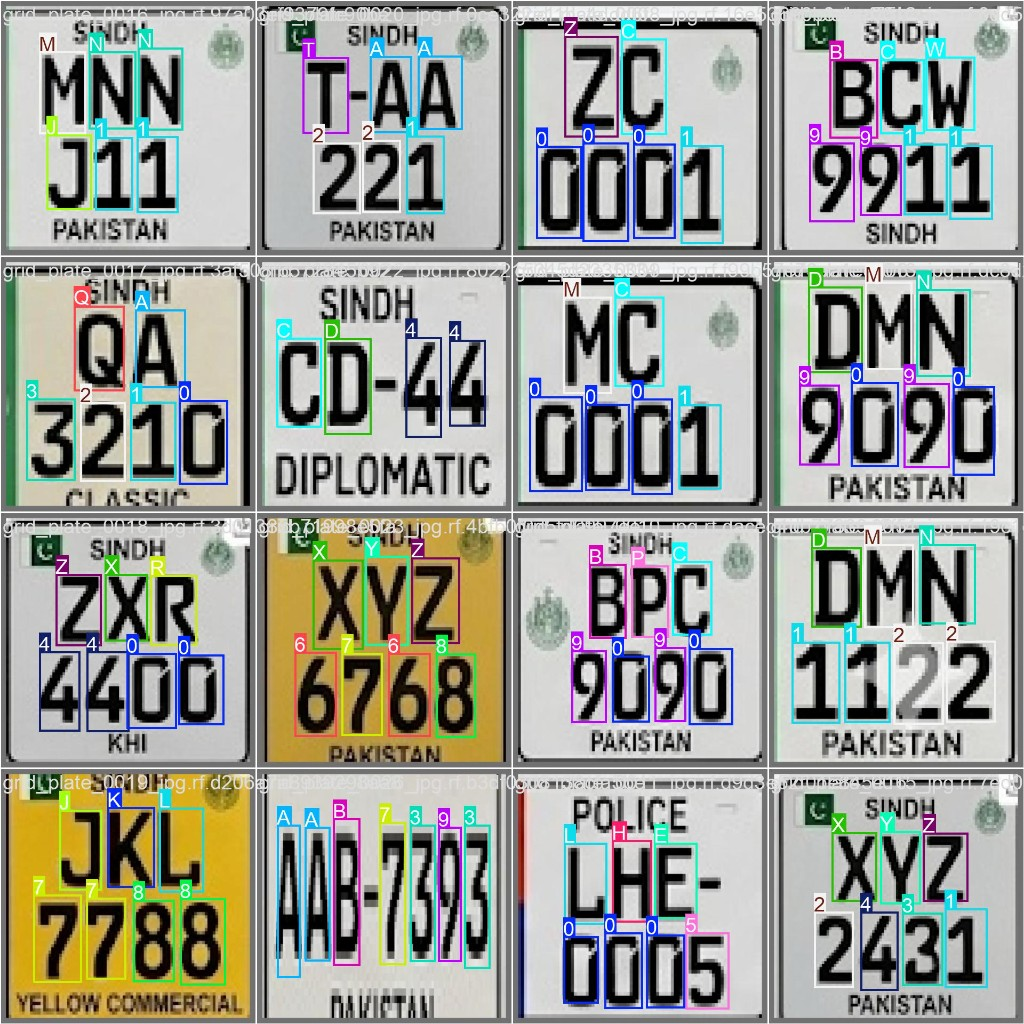
\includegraphics[width=\textwidth,keepaspectratio]{lpr_char/ocr_val_batch_labels.png}
\caption{Character validation batch mosaic with class-coloured glyph boxes on plate crops.}
\label{fig:ocr_val}
\end{figure*}
\FloatBarrier

\begin{figure*}[!htbp]
\centering
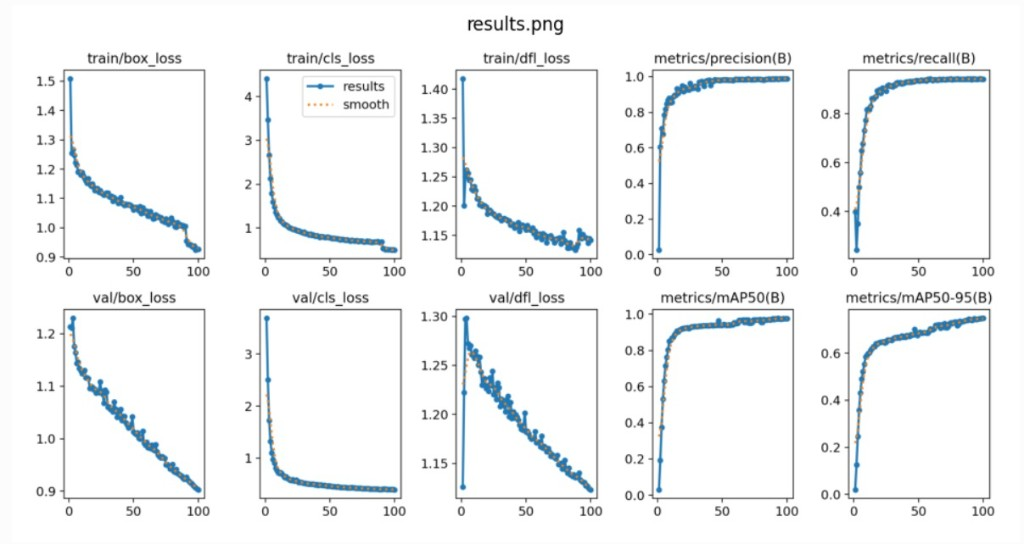
\includegraphics[width=\textwidth,keepaspectratio]{lpr_char/ocr_training_results.png}
\caption{YOLOv8n character detector training curves over 100 epochs.}
\label{fig:ocr_train}
\end{figure*}
\FloatBarrier

\begin{figure*}[!htbp]
\centering
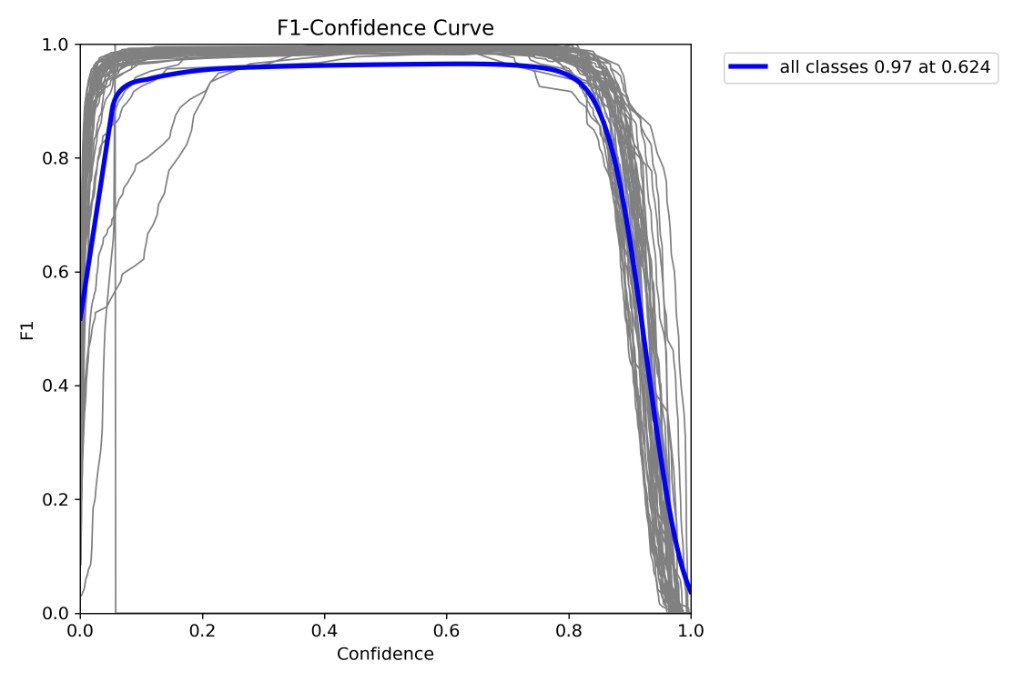
\includegraphics[width=\textwidth,keepaspectratio]{lpr_char/ocr_boxF1_curve.png}
\caption{Character detector F1--confidence curve (38 classes).}
\label{fig:ocr_f1}
\end{figure*}
\FloatBarrier

\begin{figure*}[!htbp]
\centering
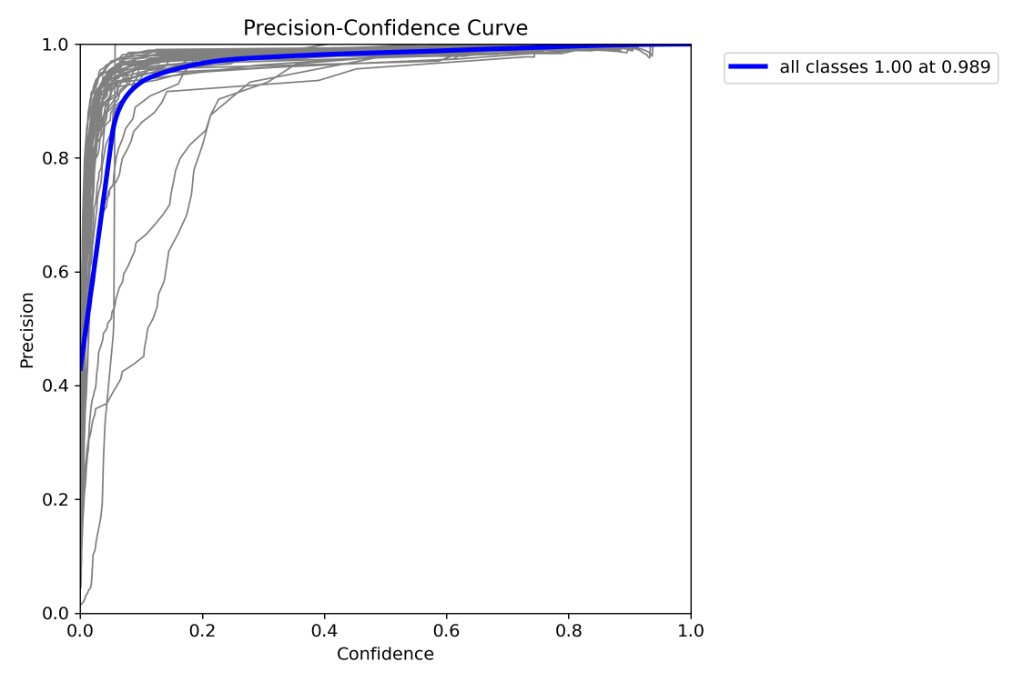
\includegraphics[width=\textwidth,keepaspectratio]{lpr_char/ocr_boxP_curve.png}
\caption{Character detector precision--confidence curve.}
\label{fig:ocr_p}
\end{figure*}
\FloatBarrier

\begin{figure*}[!htbp]
\centering
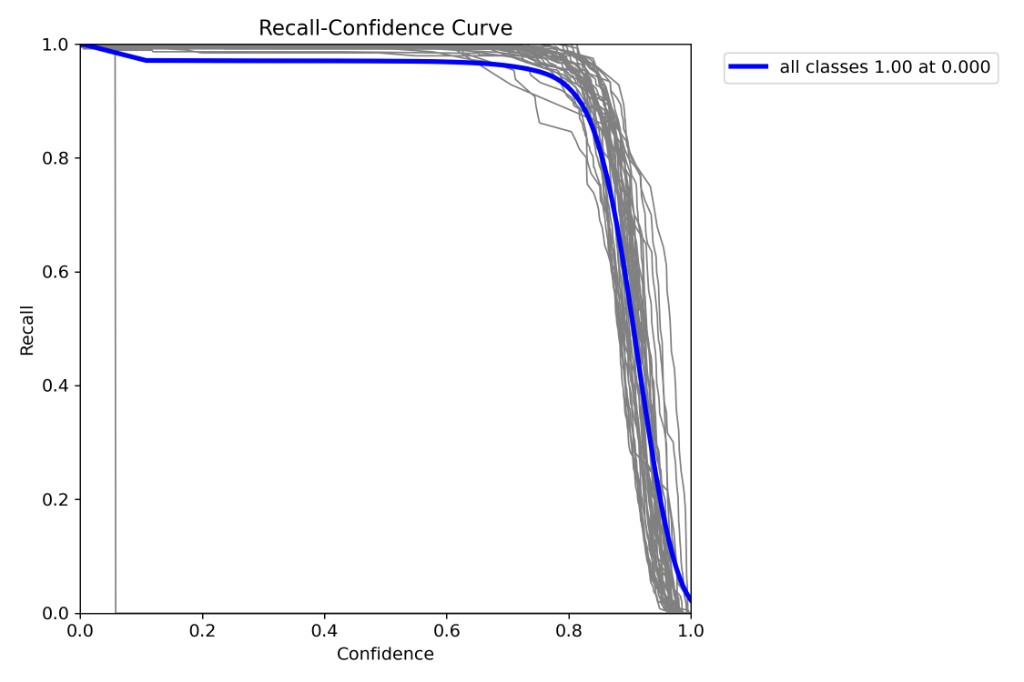
\includegraphics[width=\textwidth,keepaspectratio]{lpr_char/ocr_boxR_curve.png}
\caption{Character detector recall--confidence curve.}
\label{fig:ocr_r}
\end{figure*}
\FloatBarrier

\begin{figure*}[!htbp]
\centering
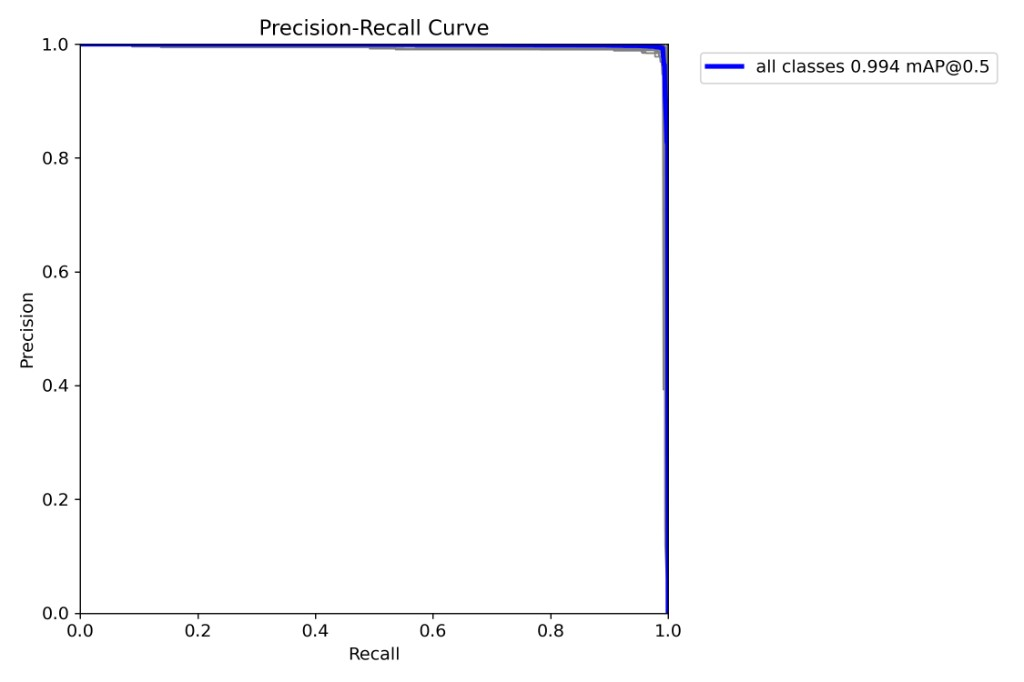
\includegraphics[width=\textwidth,keepaspectratio]{lpr_char/ocr_boxPR_curve.png}
\caption{Character detector precision--recall curve (mAP@0.5).}
\label{fig:ocr_pr}
\end{figure*}
\FloatBarrier

\begin{figure*}[!htbp]
\centering
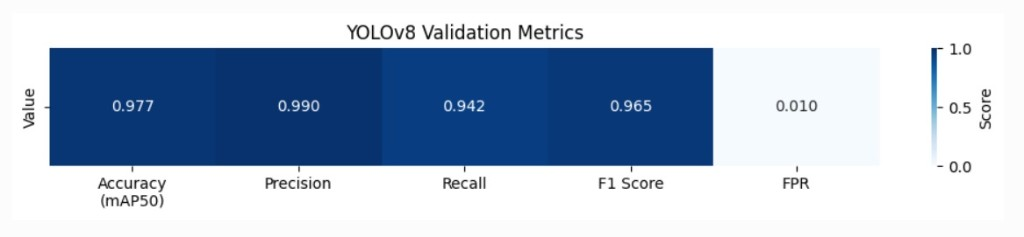
\includegraphics[width=\textwidth,keepaspectratio]{lpr_char/ocr_metrics_heatmap.png}
\caption{Character recognition metrics heatmap at epoch 100 (mAP@0.5 0.977, P 0.990, R 0.942; mirrored validation).}
\label{fig:ocr_heat}
\end{figure*}
\FloatBarrier

\begin{figure*}[!htbp]
\centering
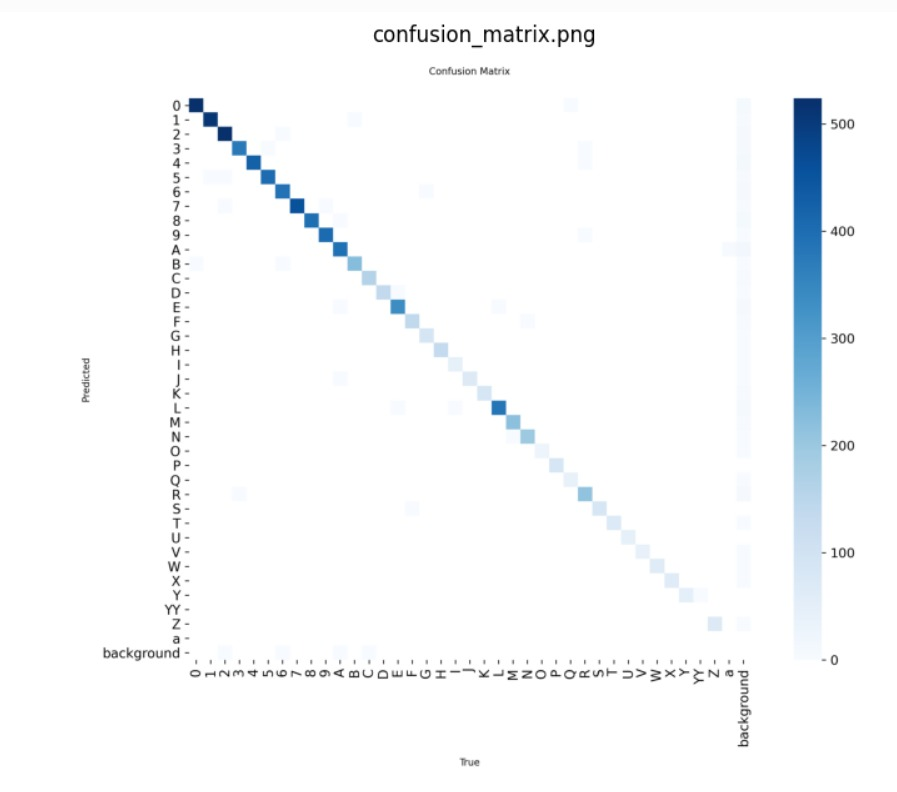
\includegraphics[width=\textwidth,keepaspectratio]{lpr_char/ocr_confusion_matrix.png}
\caption{Character recognition confusion matrix (counts) over 38 classes.}
\label{fig:ocr_cm}
\end{figure*}
\FloatBarrier

\begin{figure*}[!htbp]
\centering
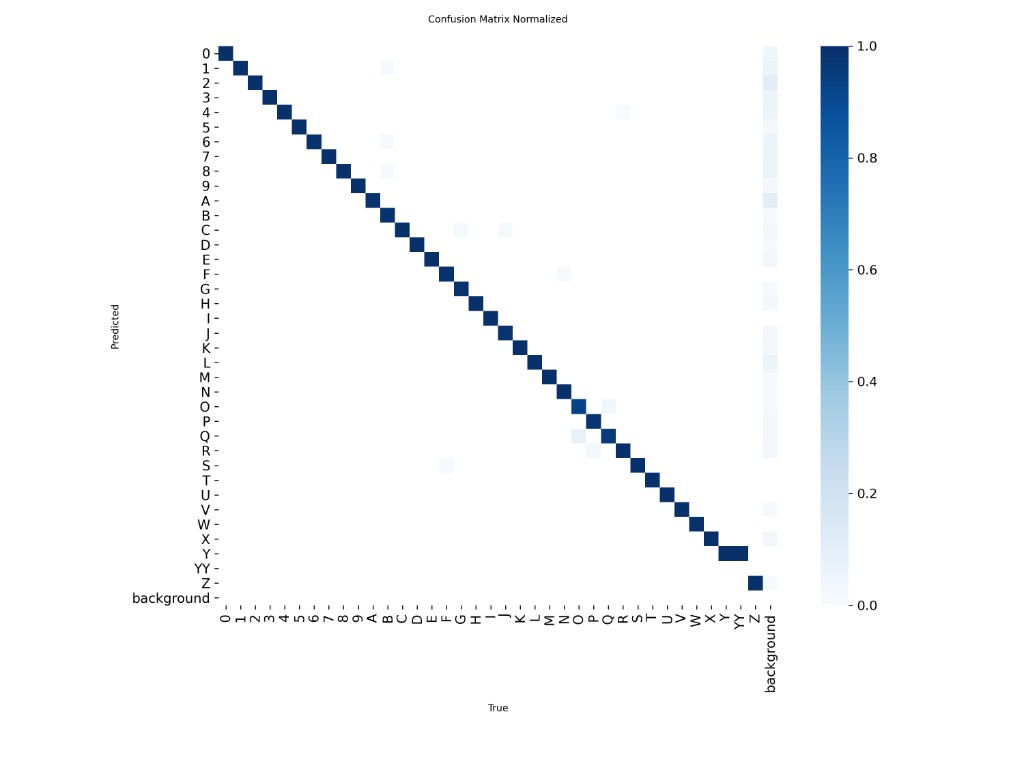
\includegraphics[width=\textwidth,keepaspectratio]{lpr_char/ocr_confusion_normalized.png}
\caption{Character recognition row-normalized confusion matrix over 38 classes.}
\label{fig:ocr_cmn}
\end{figure*}
\FloatBarrier

\begin{figure*}[!htbp]
\centering
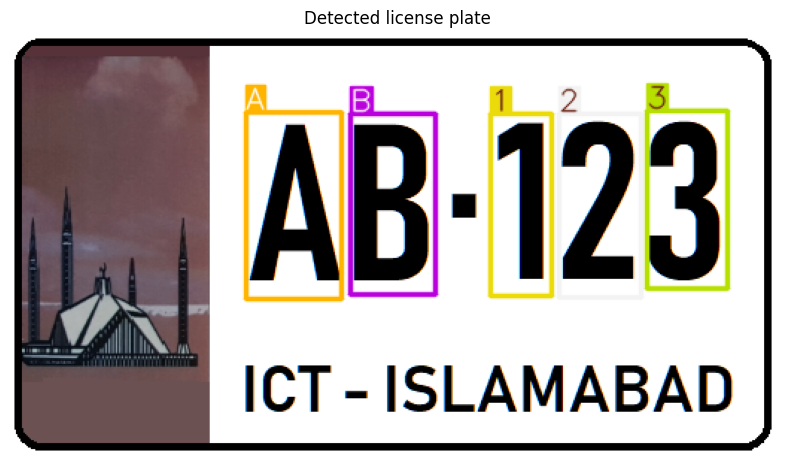
\includegraphics[width=\textwidth,keepaspectratio]{lpr_char/ocr_qual_islamabad.png}
\caption{Qualitative character localization on an ICT/Islamabad-style plate crop.}
\label{fig:ocr_isb}
\end{figure*}
\FloatBarrier

\begin{figure*}[!htbp]
\centering
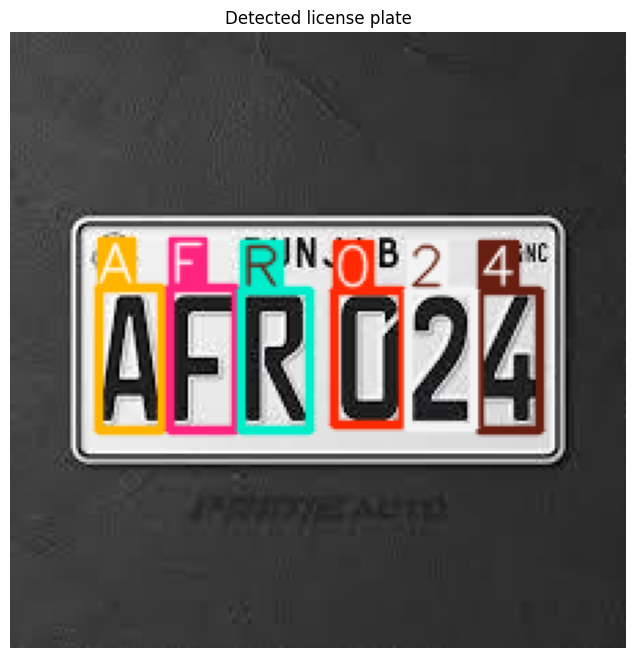
\includegraphics[width=\textwidth,keepaspectratio]{lpr_char/ocr_qual_punjab_afr.png}
\caption{Qualitative character localization on a Punjab plate (AFR-style layout).}
\label{fig:ocr_punafr}
\end{figure*}
\FloatBarrier

\begin{figure*}[!htbp]
\centering
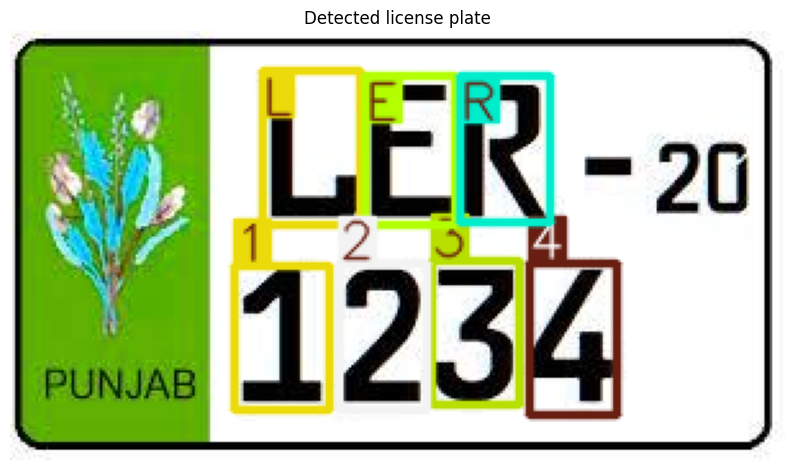
\includegraphics[width=\textwidth,keepaspectratio]{lpr_char/ocr_qual_punjab_ler.png}
\caption{Qualitative character localization on Punjab plate LER-1234.}
\label{fig:ocr_ler}
\end{figure*}
\FloatBarrier

\begin{figure*}[!htbp]
\centering
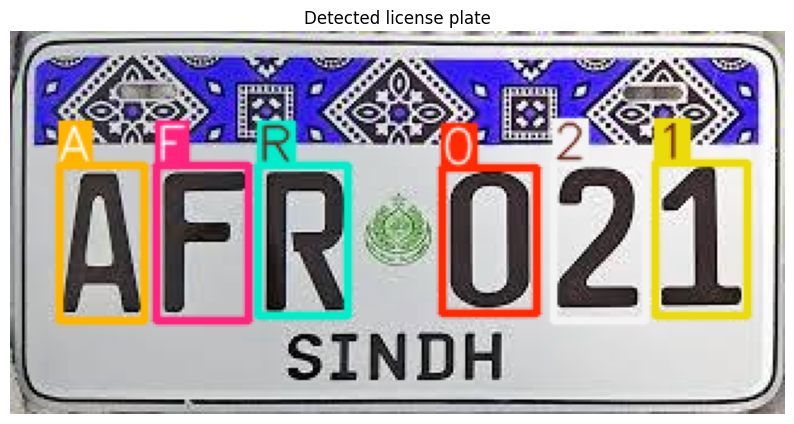
\includegraphics[width=\textwidth,keepaspectratio]{lpr_char/ocr_qual_sindh_afr021.png}
\caption{Qualitative character localization on Sindh plate AFR-021.}
\label{fig:ocr_afr021}
\end{figure*}
\FloatBarrier

\begin{figure*}[!htbp]
\centering
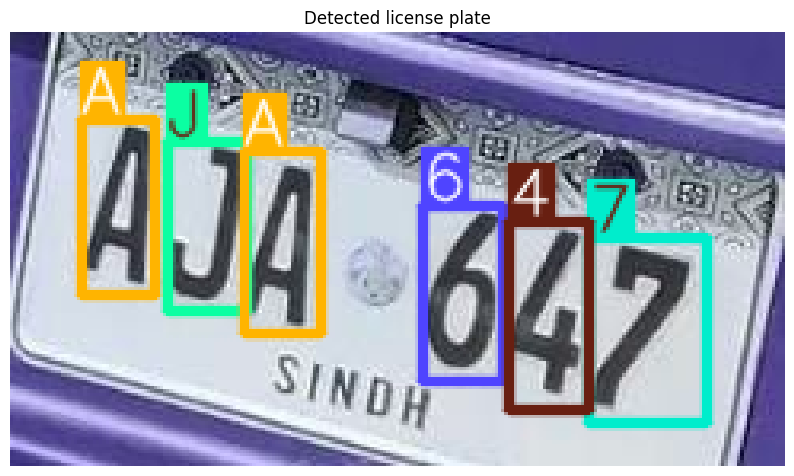
\includegraphics[width=\textwidth,keepaspectratio]{lpr_char/ocr_qual_sindh_aja.png}
\caption{Qualitative character localization on a Sindh plate with emblem spacing.}
\label{fig:ocr_aja}
\end{figure*}
\FloatBarrier

\begin{figure*}[!htbp]
\centering
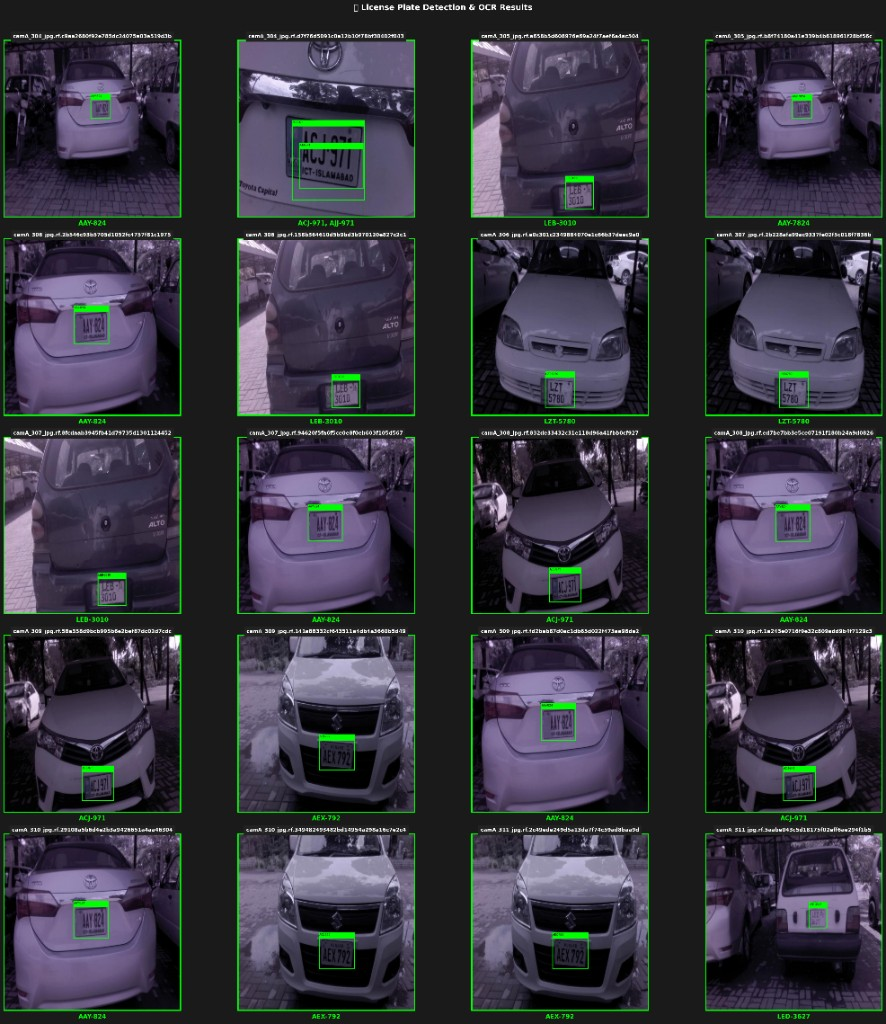
\includegraphics[width=\textwidth,keepaspectratio]{lpr_char/ocr_e2e_plate_grid.png}
\caption{End-to-end plate detection and reconstructed OCR strings on sample vehicles.}
\label{fig:ocr_e2e}
\end{figure*}
\FloatBarrier

\subsection{Vehicle Make and Model Recognition Figures}
Figures~\ref{fig:vmmr_01}--\ref{fig:vmmr_cm245} present EfficientNet-B4 diagnostics and held-out overlays. Held-out test metrics are Top-1 96.24\%, Top-5 99.39\%, and macro F1 96.18\%.

\begin{figure*}[!htbp]
\centering
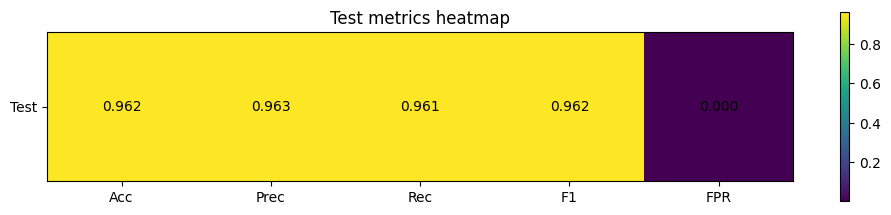
\includegraphics[width=\textwidth,keepaspectratio]{vmmr/vmmr_01.png}
\caption{VMMR test-metrics heatmap (accuracy, precision, recall, F1, and related scalars).}
\label{fig:vmmr_01}
\end{figure*}
\FloatBarrier

\begin{figure*}[!htbp]
\centering
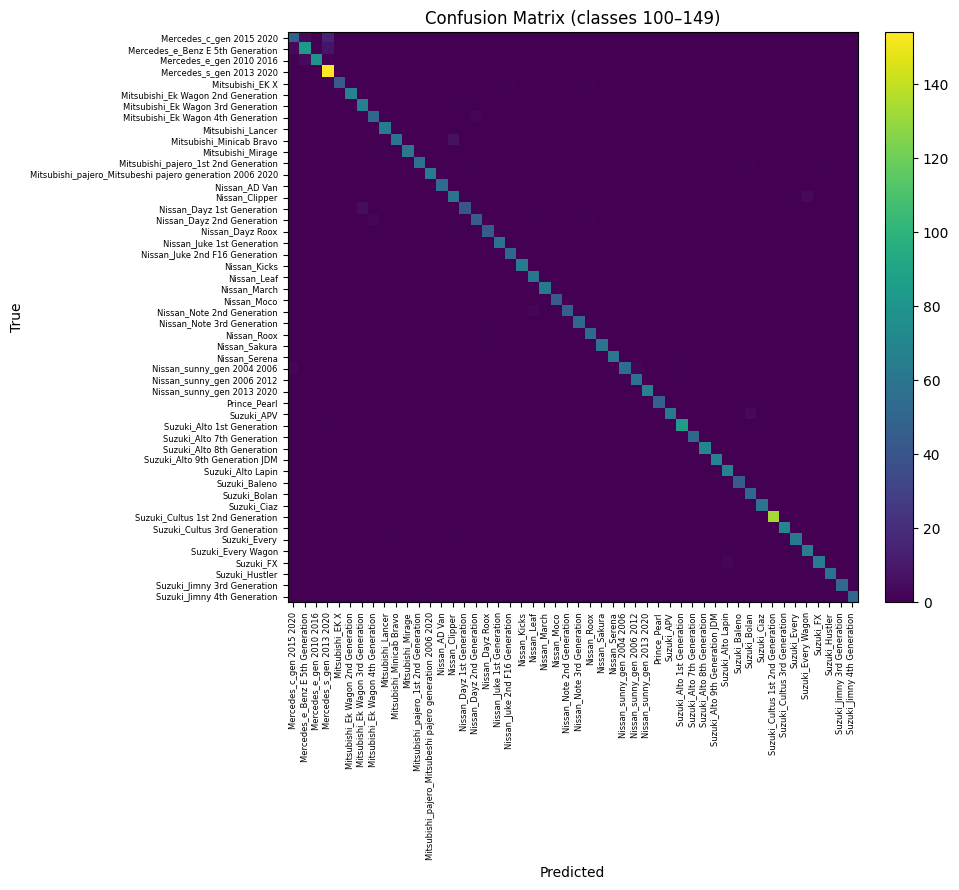
\includegraphics[width=\textwidth,keepaspectratio]{vmmr/vmmr_02.png}
\caption{VMMR confusion-matrix tile for classes 100--149.}
\label{fig:vmmr_02}
\end{figure*}
\FloatBarrier

\begin{figure*}[!htbp]
\centering
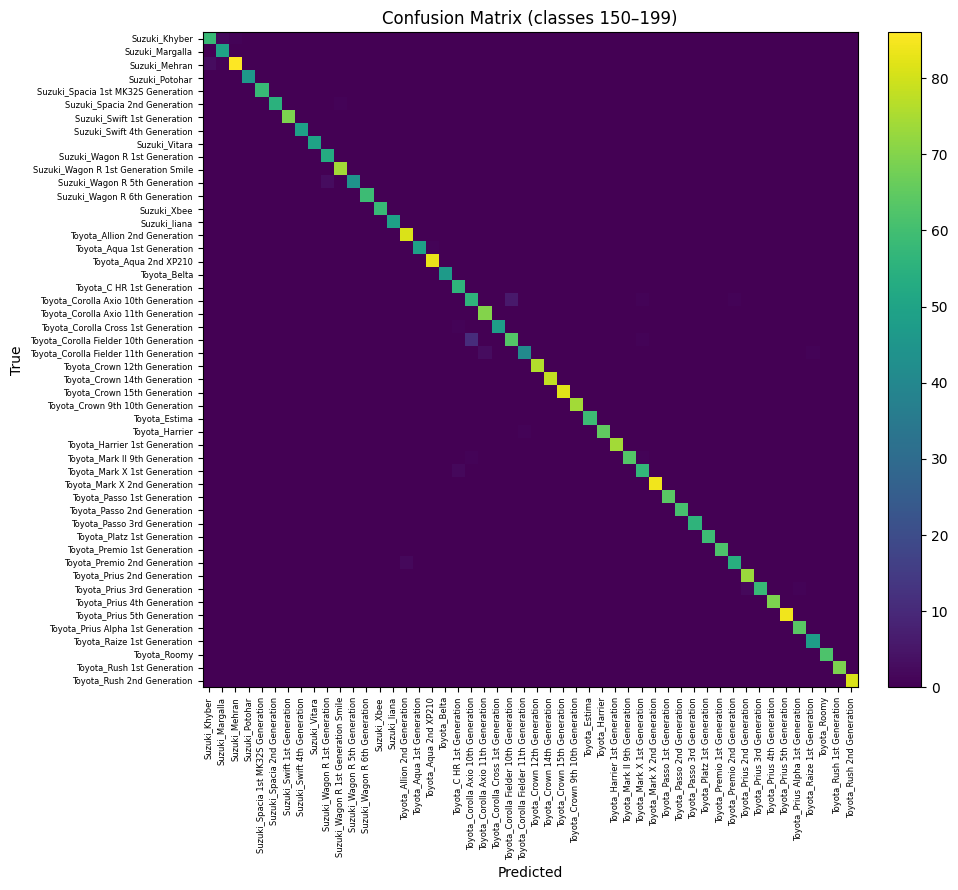
\includegraphics[width=\textwidth,keepaspectratio]{vmmr/vmmr_03.png}
\caption{VMMR confusion-matrix tile for classes 150--199.}
\label{fig:vmmr_03}
\end{figure*}
\FloatBarrier

\begin{figure*}[!htbp]
\centering
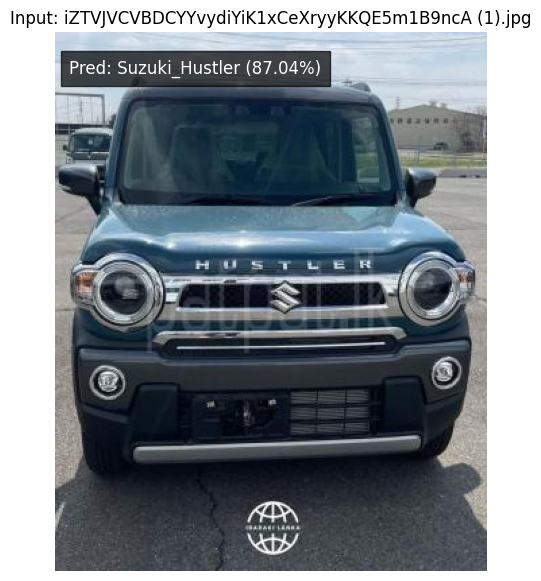
\includegraphics[width=\textwidth,keepaspectratio]{vmmr/vmmr_04.png}
\caption{Held-out VMMR inference: Suzuki Hustler (87.04\%).}
\label{fig:vmmr_04}
\end{figure*}
\FloatBarrier

\begin{figure*}[!htbp]
\centering
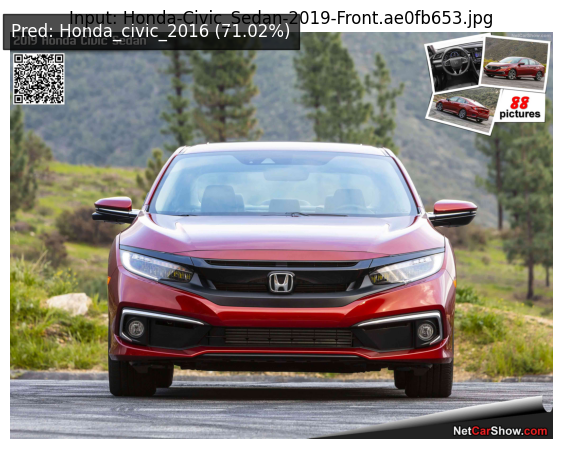
\includegraphics[width=\textwidth,keepaspectratio]{vmmr/vmmr_05.png}
\caption{Held-out VMMR inference: Honda Civic 2016 (71.02\%).}
\label{fig:vmmr_05}
\end{figure*}
\FloatBarrier

\begin{figure*}[!htbp]
\centering
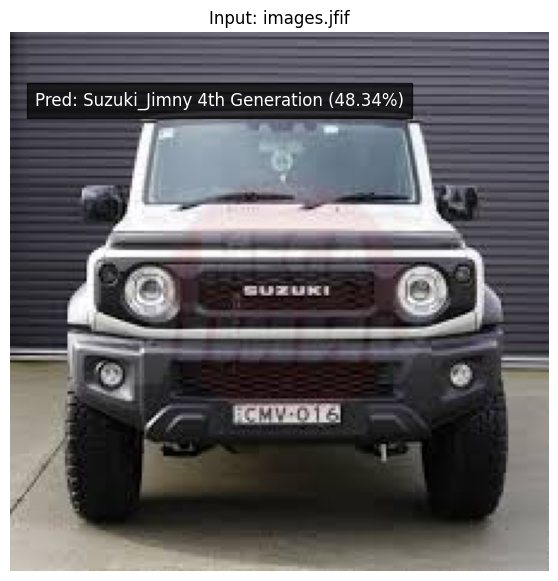
\includegraphics[width=\textwidth,keepaspectratio]{vmmr/vmmr_06.png}
\caption{Held-out VMMR inference: Suzuki Jimny 4th Gen (48.34\%).}
\label{fig:vmmr_06}
\end{figure*}
\FloatBarrier

\begin{figure*}[!htbp]
\centering
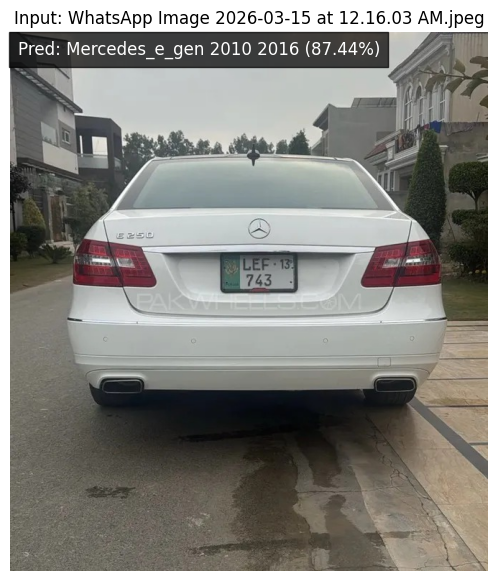
\includegraphics[width=\textwidth,keepaspectratio]{vmmr/vmmr_07.png}
\caption{Held-out VMMR inference: Mercedes E-Class sedan (87.44\%).}
\label{fig:vmmr_07}
\end{figure*}
\FloatBarrier

\begin{figure*}[!htbp]
\centering
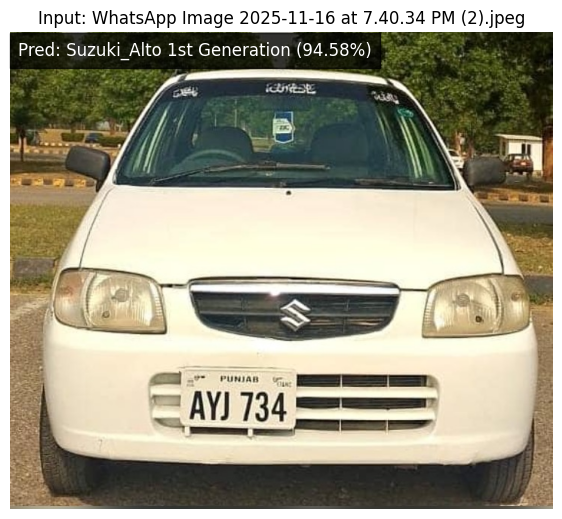
\includegraphics[width=\textwidth,keepaspectratio]{vmmr/vmmr_08.png}
\caption{Held-out VMMR inference: Suzuki Alto 1st Gen (94.58\%).}
\label{fig:vmmr_08}
\end{figure*}
\FloatBarrier

\begin{figure*}[!htbp]
\centering
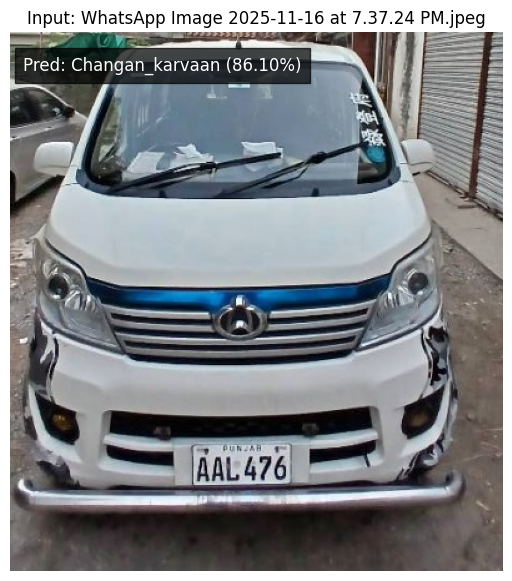
\includegraphics[width=\textwidth,keepaspectratio]{vmmr/vmmr_09.png}
\caption{Held-out VMMR inference: Changan Karvaan (86.10\%).}
\label{fig:vmmr_09}
\end{figure*}
\FloatBarrier

\begin{figure*}[!htbp]
\centering
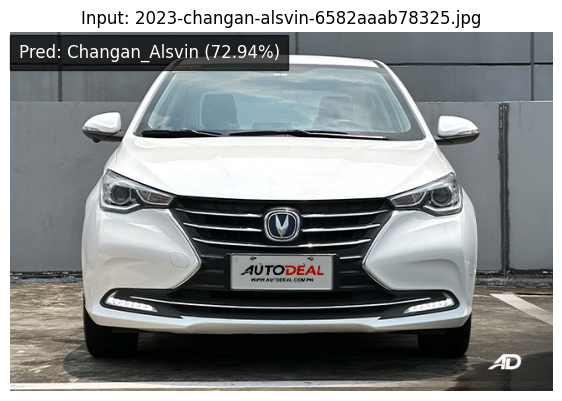
\includegraphics[width=\textwidth,keepaspectratio]{vmmr/vmmr_10.png}
\caption{Held-out VMMR inference: Changan Alsvin (72.94\%).}
\label{fig:vmmr_10}
\end{figure*}
\FloatBarrier

\begin{figure*}[!htbp]
\centering
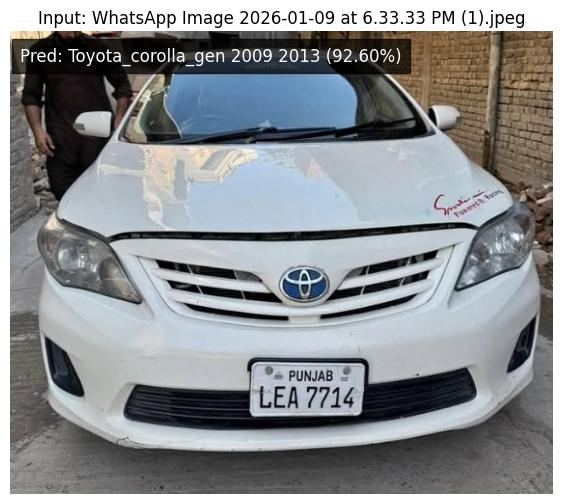
\includegraphics[width=\textwidth,keepaspectratio]{vmmr/vmmr_11.png}
\caption{Held-out VMMR inference: Toyota Corolla 2009--2013 (92.60\%).}
\label{fig:vmmr_11}
\end{figure*}
\FloatBarrier

\begin{figure*}[!htbp]
\centering
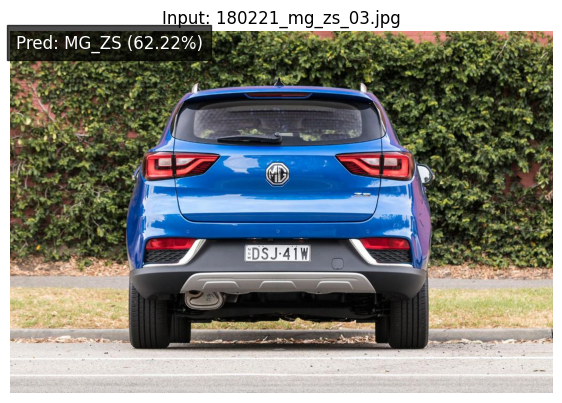
\includegraphics[width=\textwidth,keepaspectratio]{vmmr/vmmr_12.png}
\caption{Held-out VMMR inference: MG ZS SUV (62.22\%).}
\label{fig:vmmr_12}
\end{figure*}
\FloatBarrier

\begin{figure*}[!htbp]
\centering
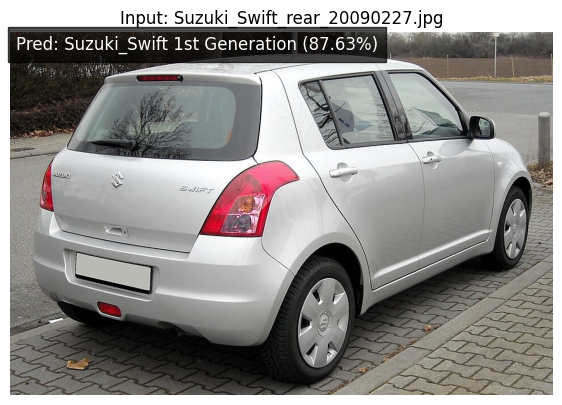
\includegraphics[width=\textwidth,keepaspectratio]{vmmr/vmmr_13.png}
\caption{Held-out VMMR inference: Suzuki Swift 1st Gen (87.63\%).}
\label{fig:vmmr_13}
\end{figure*}
\FloatBarrier

\begin{figure*}[!htbp]
\centering
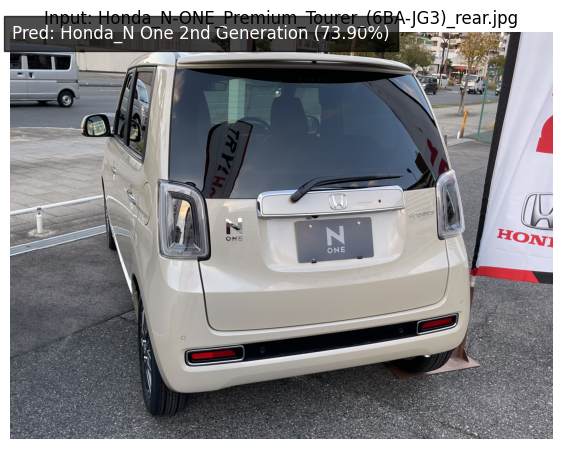
\includegraphics[width=\textwidth,keepaspectratio]{vmmr/vmmr_14.png}
\caption{Held-out VMMR inference: Honda N-One 2nd Gen (73.90\%).}
\label{fig:vmmr_14}
\end{figure*}
\FloatBarrier

\begin{figure*}[!htbp]
\centering
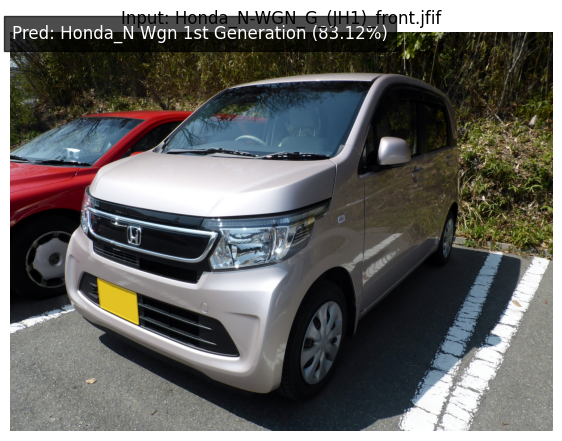
\includegraphics[width=\textwidth,keepaspectratio]{vmmr/vmmr_15.png}
\caption{Held-out VMMR inference: Honda N-Wgn 1st Gen (83.12\%).}
\label{fig:vmmr_15}
\end{figure*}
\FloatBarrier

\begin{figure*}[!htbp]
\centering
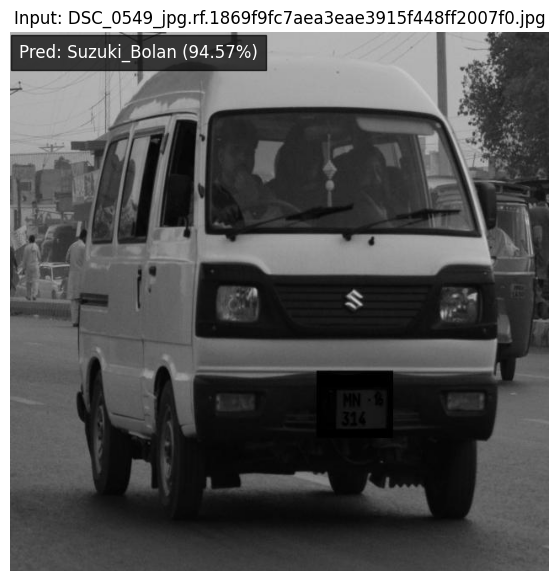
\includegraphics[width=\textwidth,keepaspectratio]{vmmr/vmmr_16.png}
\caption{Held-out VMMR inference: Suzuki Bolan (94.57\%).}
\label{fig:vmmr_16}
\end{figure*}
\FloatBarrier

\begin{figure*}[!htbp]
\centering
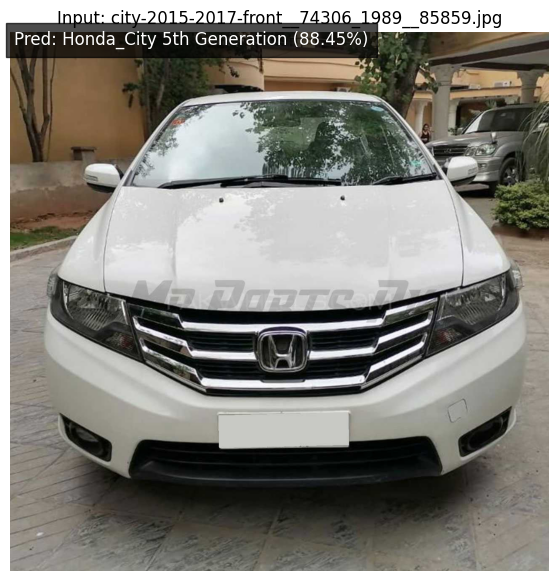
\includegraphics[width=\textwidth,keepaspectratio]{vmmr/vmmr_17.png}
\caption{Held-out VMMR inference: Honda City 5th Gen (88.45\%).}
\label{fig:vmmr_17}
\end{figure*}
\FloatBarrier

\begin{figure*}[!htbp]
\centering
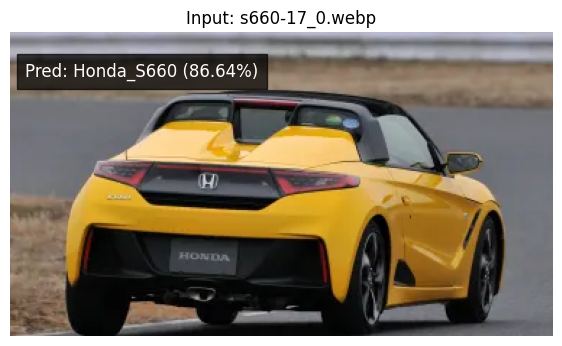
\includegraphics[width=\textwidth,keepaspectratio]{vmmr/vmmr_18.png}
\caption{Held-out VMMR inference: Honda S660 (86.64\%).}
\label{fig:vmmr_18}
\end{figure*}
\FloatBarrier

\begin{figure*}[!htbp]
\centering
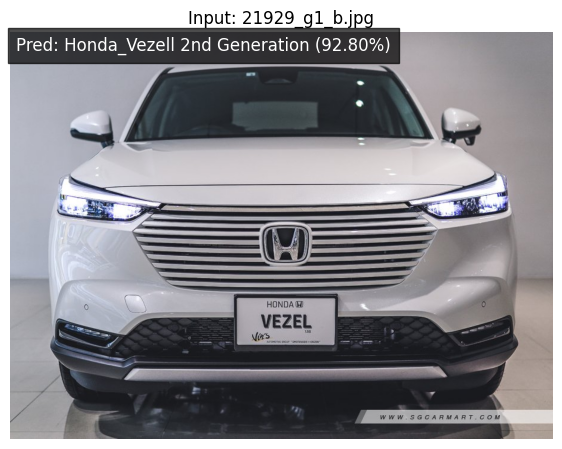
\includegraphics[width=\textwidth,keepaspectratio]{vmmr/vmmr_19.png}
\caption{Held-out VMMR inference: Honda Vezel 2nd Gen (92.80\%).}
\label{fig:vmmr_19}
\end{figure*}
\FloatBarrier

\begin{figure*}[!htbp]
\centering
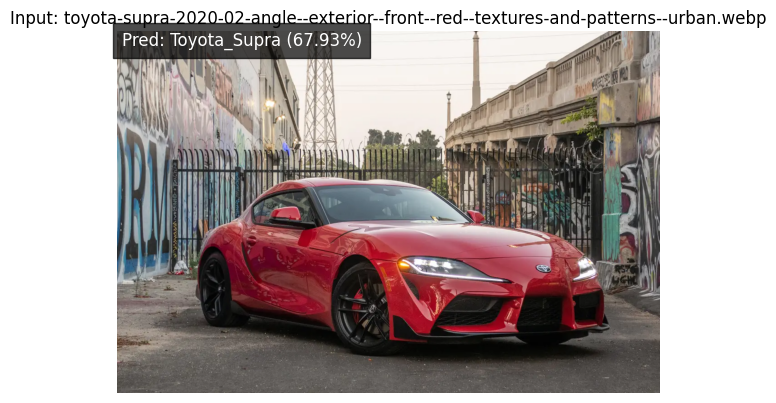
\includegraphics[width=\textwidth,keepaspectratio]{vmmr/vmmr_20.png}
\caption{Held-out VMMR inference: Toyota Supra (67.93\%).}
\label{fig:vmmr_20}
\end{figure*}
\FloatBarrier

\begin{figure*}[!htbp]
\centering
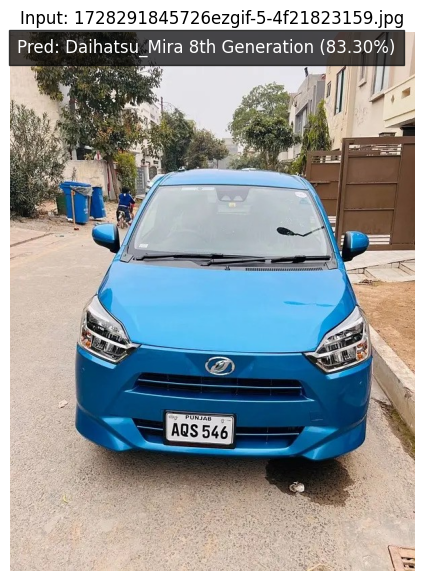
\includegraphics[width=\textwidth,keepaspectratio]{vmmr/vmmr_21.png}
\caption{Held-out VMMR inference: Daihatsu Mira 8th Gen (83.30\%).}
\label{fig:vmmr_21}
\end{figure*}
\FloatBarrier

\begin{figure*}[!htbp]
\centering
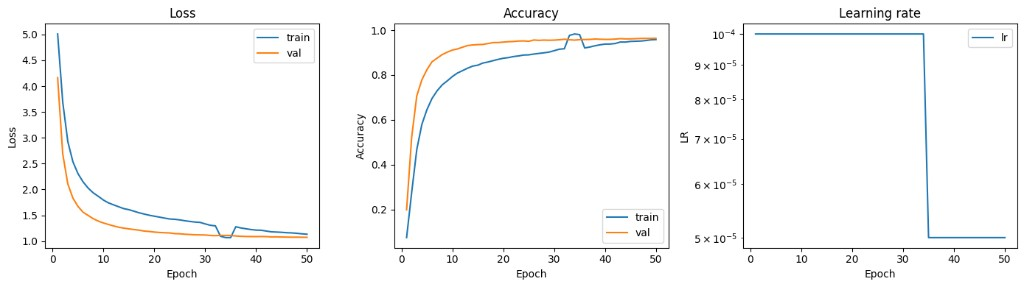
\includegraphics[width=\textwidth,keepaspectratio]{vmmr/vmmr_22.png}
\caption{VMMR training curves: loss, accuracy, and learning rate over 50 epochs.}
\label{fig:vmmr_22}
\end{figure*}
\FloatBarrier

\begin{figure*}[!htbp]
\centering
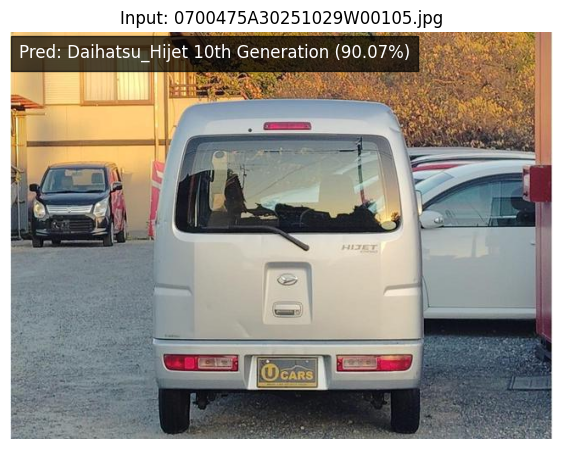
\includegraphics[width=\textwidth,keepaspectratio]{vmmr/vmmr_23.png}
\caption{Held-out VMMR inference: Daihatsu Hijet 10th Gen (90.07\%).}
\label{fig:vmmr_23}
\end{figure*}
\FloatBarrier

\begin{figure*}[!htbp]
\centering
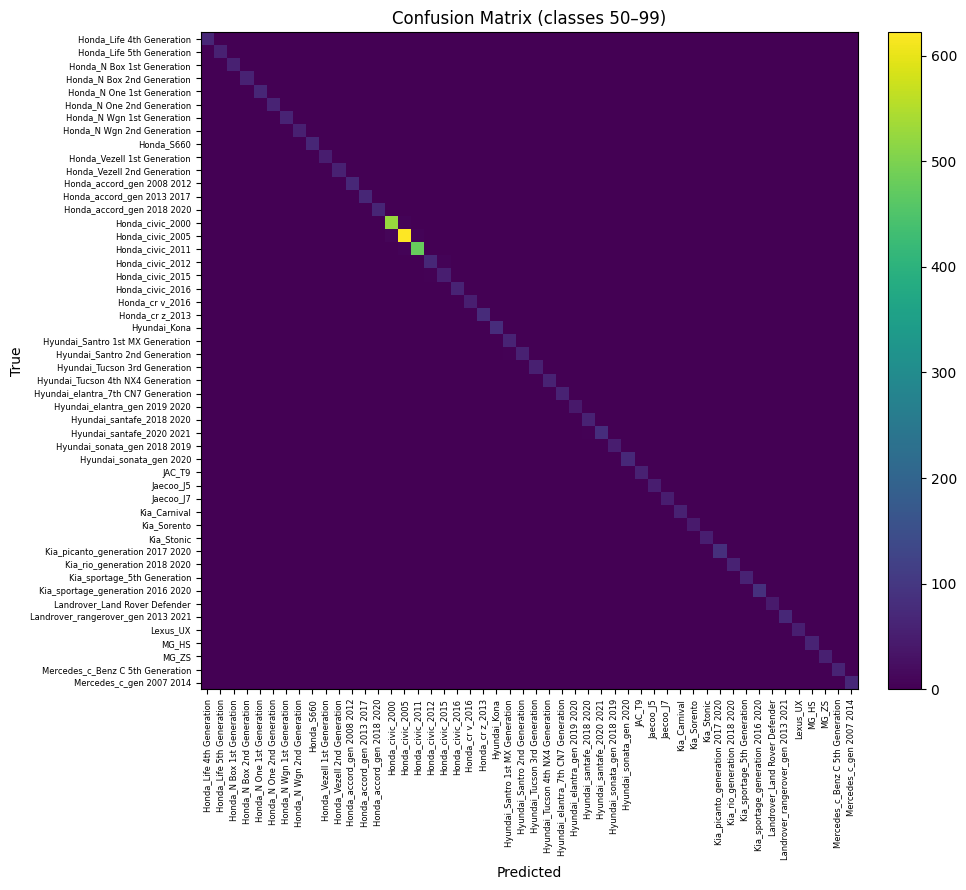
\includegraphics[width=\textwidth,keepaspectratio]{vmmr/vmmr_24.png}
\caption{VMMR confusion-matrix tile for classes 136--162.}
\label{fig:vmmr_24}
\end{figure*}
\FloatBarrier

\begin{figure*}[!htbp]
\centering
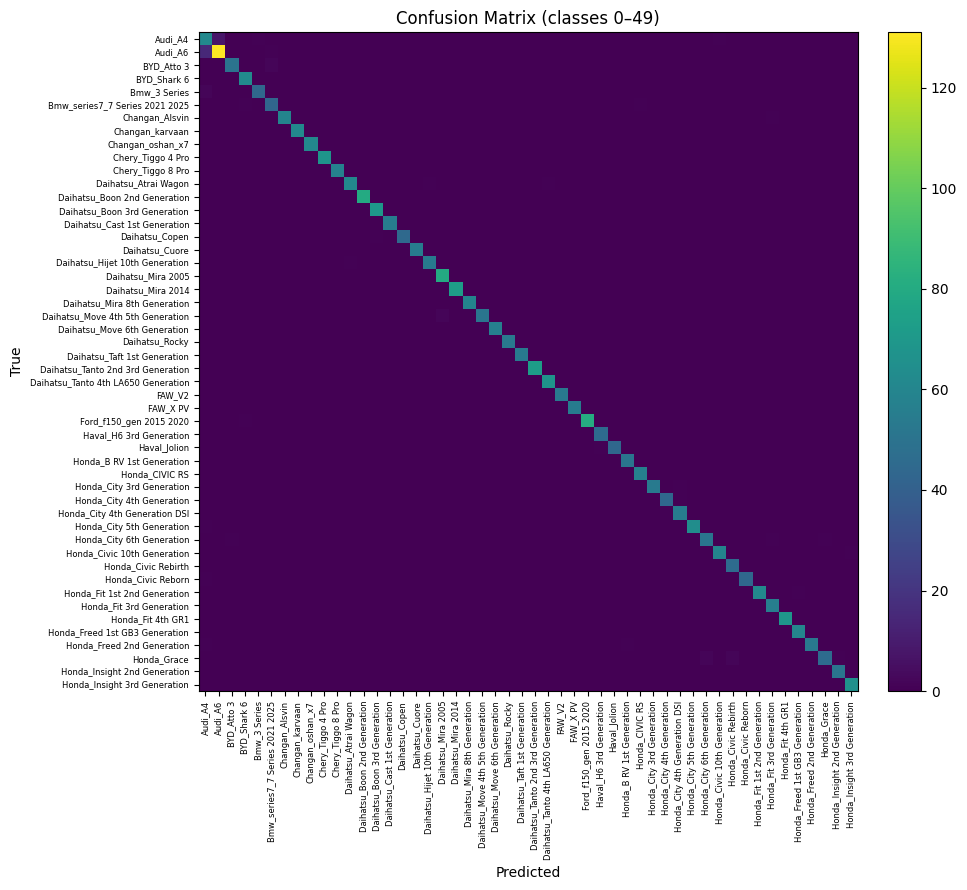
\includegraphics[width=\textwidth,keepaspectratio]{vmmr/vmmr_25.png}
\caption{VMMR confusion-matrix tile for classes 0--43.}
\label{fig:vmmr_25}
\end{figure*}
\FloatBarrier

\begin{figure*}[!htbp]
\centering
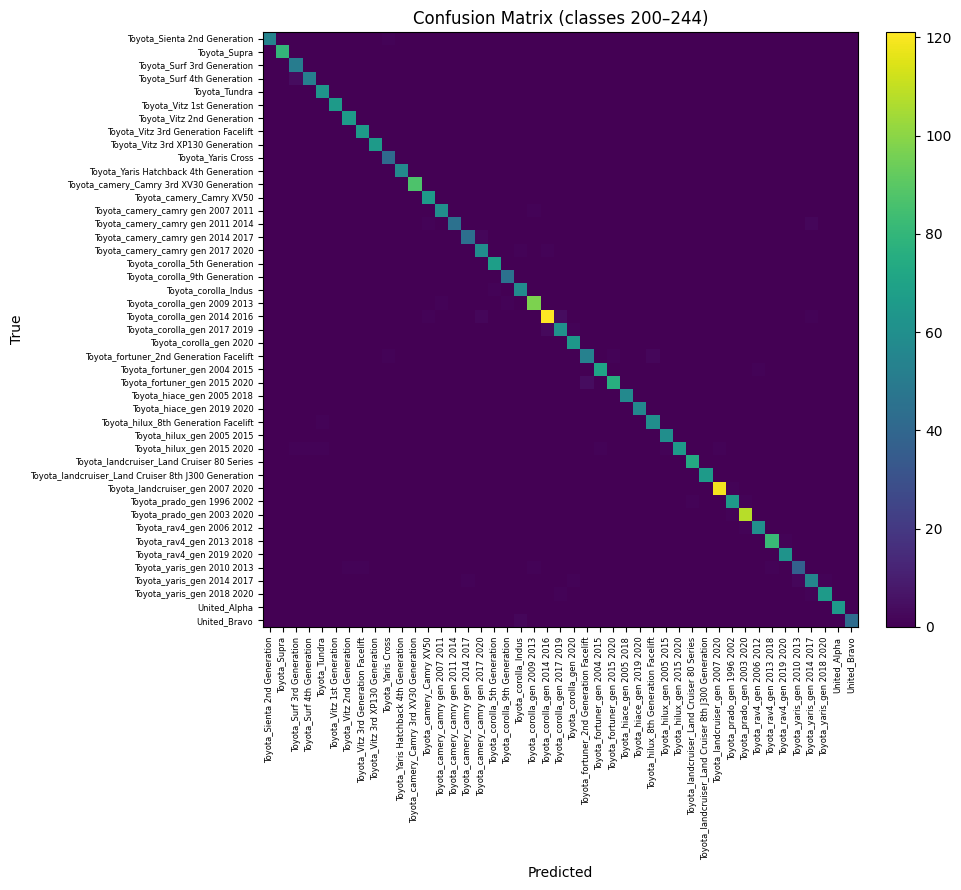
\includegraphics[width=\textwidth,keepaspectratio]{vmmr/vmmr_26.png}
\caption{VMMR confusion-matrix tile for classes 200--244.}
\label{fig:vmmr_26}
\end{figure*}
\FloatBarrier

\begin{figure*}[!htbp]
\centering
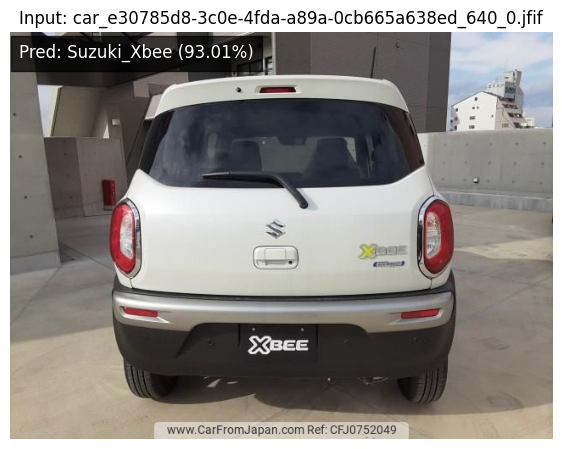
\includegraphics[width=\textwidth,keepaspectratio]{vmmr/vmmr_27.png}
\caption{Held-out VMMR inference: Suzuki Xbee (93.01\%).}
\label{fig:vmmr_27}
\end{figure*}
\FloatBarrier

\begin{figure*}[!htbp]
\centering
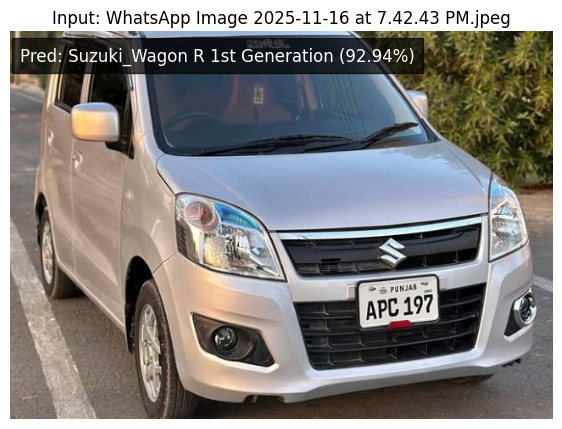
\includegraphics[width=\textwidth,keepaspectratio]{vmmr/vmmr_28.png}
\caption{VMMR Top-5 prediction montage on held-out samples.}
\label{fig:vmmr_28}
\end{figure*}
\FloatBarrier

\begin{figure*}[!htbp]
\centering
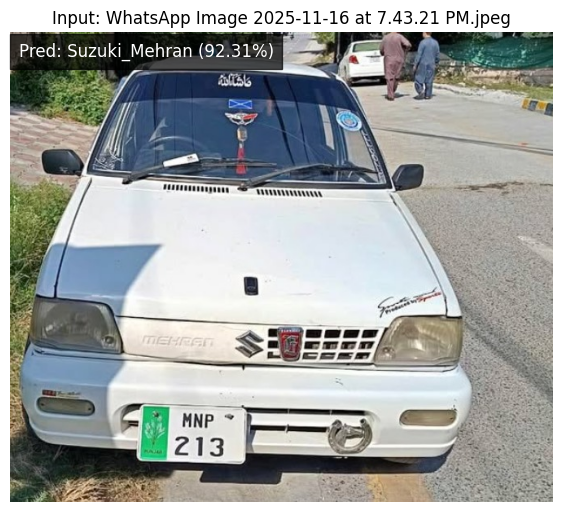
\includegraphics[width=\textwidth,keepaspectratio]{vmmr/vmmr_29.png}
\caption{VMMR macro false-positive-rate summary heatmap.}
\label{fig:vmmr_29}
\end{figure*}
\FloatBarrier

\begin{figure*}[!htbp]
\centering
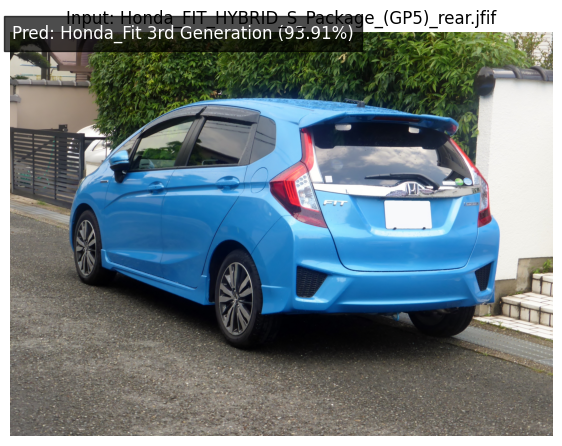
\includegraphics[width=\textwidth,keepaspectratio]{vmmr/vmmr_30.png}
\caption{VMMR per-class precision strip highlighting tail classes.}
\label{fig:vmmr_30}
\end{figure*}
\FloatBarrier

\begin{figure*}[!htbp]
\centering
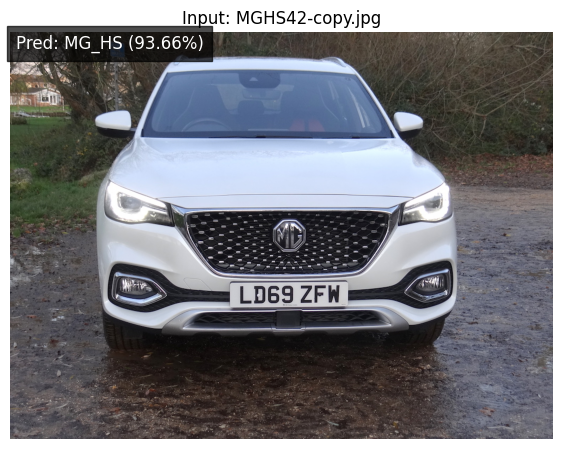
\includegraphics[width=\textwidth,keepaspectratio]{vmmr/vmmr_31.png}
\caption{Printed aggregate VMMR test metrics (Top-1 and macro-F1 readouts).}
\label{fig:vmmr_31}
\end{figure*}
\FloatBarrier

\begin{figure*}[!htbp]
\centering
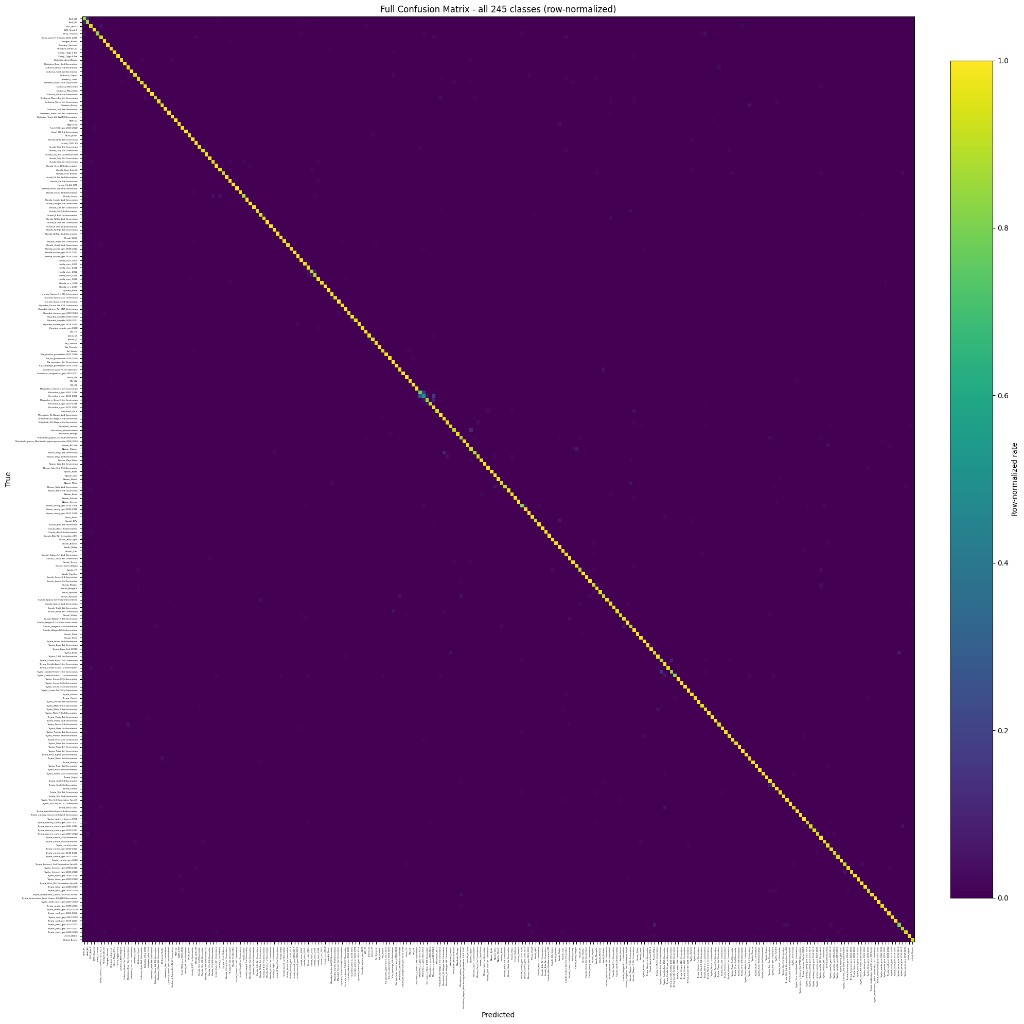
\includegraphics[width=\textwidth,keepaspectratio]{vmmr/vmmr_confusion_matrix_245.png}
\caption{Full row-normalized confusion matrix for all 245 VMMR classes on the held-out test split (EfficientNet-B4).}
\label{fig:vmmr_cm245}
\end{figure*}
\FloatBarrier

\section{Discussion}
\label{sec:disc}
Plate detection mAP@0.5 of 98.07\% indicates reliable localization on Roboflow v1. Character metrics must be discounted because validation mirrored training. VMMR Top-1 of 96.24\% on 17{,}254 images is the strongest held-out classification result; residual errors concentrate on visually similar sibling-year classes (Fig.~\ref{fig:vmmr_cm245}). Dual verification addresses plate swapping. Orange Pi latency shows VMMR dominates runtime while staying under the $<$2\,s objective (Fig.~\ref{fig:edge_lat}).

\subsection{Limitations}
Region generalization is untested outside Pakistani plates/vehicles; character validation is not disjoint; snow/smog/extreme glare remain weak; weather branch selection is not sensor-driven; industrial barrier actuation is out of scope; weather-branch string accuracy is qualitative.

\section{Conclusion and Future Work}
\label{sec:conc}
This FYP implemented an Automatic Vehicle Gate Access System coupling weather-aware restoration, YOLOv8n LPR, EfficientNet-B4 VMMR (245 classes), dual-modality authorization, Orange Pi edge deployment, and a Vercel React dashboard. Reported results: 98.07\% mAP@0.5 (LPD), 97.7\% mAP@0.5 (characters, mirrored val), 96.24\% Top-1 (VMMR), and $\sim$700--1000\,ms CPU latency. Future work includes GPIO/relay barrier actuation, multi-frame voting, sensor-triggered preprocessing, persistent cloud storage, and a true character validation split.

\section*{Acknowledgment}
The authors thank Dr.\ Taimoor Naeem, Department of Computer Engineering, COMSATS University Islamabad, Lahore Campus, for supervision of this final-year project.

\clearpage
\balance
\bibliographystyle{IEEEtran}
\bibliography{references}

\end{document}
